\documentclass{statsmsc}
\usepackage{float}
\usepackage{hyperref}
\usepackage[utf8]{inputenc}
\usepackage{graphicx}
\usepackage{caption}
\usepackage{subcaption}
\usepackage{algpseudocode}
\usepackage{algorithm}
\usepackage{mathtools}
\usepackage{amsmath,amssymb}
\usepackage{nccmath}
\usepackage{siunitx}
\usepackage{listings}
\usepackage{physics}
\usepackage{tikz}
\usepackage[outline]{contour} % glow around text
\usepackage{bbm}
\usepackage[most]{tcolorbox}
\newcommand{\e}[1]{{\mathbb E}\left[ #1 \right]}
\definecolor{block-gray}{gray}{0.90}
\newtcolorbox{code}{colback=block-gray,grow to right by=-1mm,grow to left by=-1mm,boxrule=0pt,boxsep=0pt,breakable}
\lstset{
  basicstyle=\ttfamily,
  columns=fullflexible,
  frame=single,
  breaklines=true,
  postbreak=\mbox{\textcolor{red}{$\hookrightarrow$}\space},
}
\usetikzlibrary{patterns,snakes}
\usetikzlibrary{arrows.meta} % for arrow size
\contourlength{0.4pt}

\colorlet{xcol}{blue!70!black}
\colorlet{darkblue}{blue!40!black}
\colorlet{myred}{red!65!black}
\tikzstyle{mydashed}=[xcol,dashed,line width=0.25,dash pattern=on 2.2pt off 2.2pt]
\tikzstyle{axis}=[->,thick] %line width=0.6
\tikzstyle{ell}=[{Latex[length=3.3,width=2.2]}-{Latex[length=3.3,width=2.2]},line width=0.3]
\tikzstyle{dx}=[-{Latex[length=3.3,width=2.2]},darkblue,line width=0.3]
\tikzstyle{ground}=[preaction={fill,top color=black!10,bottom color=black!5,shading angle=20},
                    fill,pattern=north east lines,draw=none,minimum width=0.3,minimum height=0.6]
\tikzstyle{mass}=[line width=0.6,red!30!black,fill=red!40!black!10,rounded corners=1,
                  top color=red!40!black!20,bottom color=red!40!black!10,shading angle=20]
\tikzstyle{spring}=[line width=0.8,blue!7!black!80,snake=coil,segment amplitude=5,segment length=5,line cap=round]
\tikzset{>=latex} % for LaTeX arrow head
\tikzstyle{force}=[->,myred,very thick,line cap=round]
\def\tick#1#2{\draw[thick] (#1)++(#2:0.1) --++ (#2-180:0.2)}
\newsavebox{\overlongequation}
\newenvironment{CentreLongEquation}
 {\begin{displaymath}\begin{lrbox}{\overlongequation}$\displaystyle}
 {$\end{lrbox}\makebox[0pt]{\usebox{\overlongequation}}\end{displaymath}}


\title{Learning Invariances in Dynamical System}
\author{Cheng-Cheng Lao}
\CID{01353756}
\supervisor{Dr. Andrew Duncan and Dr. Mark van der Wilk}
\date{\today}
%For today's date, use:
%\date{\today}
\logoimg{}


% THIS IS WHERE NEW COMMANDS CAN BE DEFINED
% commands below only used in the proof; otherwise can be deleted
\newcommand{\consta}{a}
\newcommand{\X}{X}
\newcommand{\EE}[1]{ \mathrm{E} [ #1 ] }
\newcommand{\inparenth}[1]{\left( #1 \right)}

\begin{document}

% Generates the Title Page
\maketitle


% Generates plagiarism declaration
\declarationname{Cheng-Cheng Lao}
\declarationdate{\today}
\declaration 


\begin{abstract}
    ABSTRACT GOES HERE
\end{abstract}

\begin{acknowledgements}
    ANY ACKNOWLEDGEMENTS GO HERE
\end{acknowledgements}

% add glossary?

% VERY IMPORTANT
% This command switches from Roman to Arabic numbering for main part of thesis
\mainmatter


\chapter{Introduction}
Dynamical system is one of the richest theory that models the real world with wide application across all science and engineering. 
Of course, it is an interesting area of mathematics to study on its own.
In practice, it will be very valuable to be able to reliably predict the evolution of a system for many purpose; both from a theortical and practical point of view.
Recently, data intensive machine learning methods, such as deep learning, has shown some very powerful results. 
However, the amount of data required are often enormous, and that will involve lots of manual labour to label and process the data.
Sometimes, the data could be very difficult to come by.
Therefore, data efficiency is the key in the future if we wish to study more complicated systems.
Inductive bias is one way to achieve the goal.
What was usually done is to embed the inductive bias into the model in some way so that the model "understands" this knowledge before seeing the data.
Assuming the inductive bias is correct, we would expect the model to perform better, either in a data efficiency way or prediction performance way.
One very powerful inductive bias is the use of symmetry and invariances, that puts strong constraints on the model to obey.



\chapter{Background}
Here we will cover the background knowledge required to understand the remaining thesis, including Gaussian Process, dynamical systems as well as symmetry and invariances. 
This section will also cover related work in the field.


\section{Gaussian Process}
Gaussian Process (GP) can be thought of a distribution over functions. \cite{rasmussen_williams_2006}
More formally, \begin{quote}GP is a collection of random variables, any finite number of which have a joint Gaussian distribution\end{quote}
We will be able to specify a GP on $f(\mathbf{x})$ by mean function $m(\mathbf{x})=\mathbb{E}[f(\mathbf{x})]$ as well as the kernel function $k(\mathbf{x}, \mathbf{x'})=\mathbb{E}[f(\mathbf{x})-m(\mathbf{x})(f(\mathbf{x'}-m{\mathbf{x'}}))]$.
We then then write
$$
f(\mathbf{x})\sim\mathcal{GP}(m(\mathbf{x}),k(\mathbf{x},\mathbf{x'})).
$$
If we assume the signal is not noise free such that we assume a Gaussian noise $y=f+\epsilon$, where $\epsilon\sim\mathcal{N}(0, \sigma_n^2)$.
Then we will have 
An important identity we use throughout the thesis is the Gaussian conditional formula; if
$$
  \begin{bmatrix}
    x\\y
  \end{bmatrix} 
  \sim \mathcal{N}
  \left(
    \begin{bmatrix}
      \mathbf{\mu}_x\\
      \mathbf{\mu}_y
    \end{bmatrix},
    \begin{bmatrix}
      A & C \\
      C^T & B\\
    \end{bmatrix}
  \right)
$$, 
then 
\begin{equation}
  x|y\sim \mathcal{N}\left(\mathbf{\mu}_x+CB^{-1}(y-\mathbf{\mu}_y),A-CB^{-1}C^T\right)
  \label{equ:normal_condtion}
\end{equation}

\subsection{GPflow}
GPflow is used throughout the project (\cite{GPflow2017}).
It is a Python package built on TensorFlow to allow efficient and fast computation on GPUs to do GP inferences.
A particular powerful feature is that it allows the choosing of hyperparameter such as lengthscales and variance of a kernel automatic by calculating the gradient (using automatic differentiation feature of Tensorflow) and perform optimisation.
In later sections, we will need to optimise more parameters than aforementioned ones with respect to maginal likelihood objective.


\section{Dynamical Systems}
Dynamical system, which describes the evolution of a system in time, can be broadly classified to two catergories: differential equations and difference equations, with the former being continous time and the latter being discrete time. (\cite{strogatz_2019}). 
We will formalise our notion and notation using continous time (differential equation) description.
There are many real world systems that can be modelled by a dynamical system, for example a huge class of problems in engineering and physics. 
A simple example, which will also be explored later, is a damped pendulum, with equation of motion
$$
m\frac{d^2x}{dt^2}+b\frac{dx}{dt}+kx=0.
$$
In general an $n^{th}$ degree differential equations can be written as 
$$
\frac{d^{n} x}{d t^{n}}=F\left(t, x, \frac{d x}{d t}, \ldots, \frac{d^{n-1} x}{d t^{n-1}}\right),
$$
(\cite{glendinning_1994}) and we will need $n$ initial conditions to specify a solution for the differential equations.
We can also write $n^{th}$ degree ordinary differential equations (ODEs) as $n$ degree one coupled ODE. 
For example, in the above case, we can write it as 
$$
\begin{cases}
  \frac{dx}{dt} = v\\
  \frac{dv}{dt} = \frac{-bv-kx}{m}\\
\end{cases}
$$
More generally, we can write 
$$
\begin{cases}
  \dot{x}_1=f_1(x_1, \dots, x_n)\\ 
  \vdots\\
  \dot{x}_n=f_n(x_1, \dots, x_n)\\ 
\end{cases}
$$

We can then visualise the state of the system described by the $n$ variables in the "phase space", and this system will evolve or move in the phase space as time evolves. 
For instance, the damped pendulum is of degree 2 so there will be two variables describing its evolution, which in this case will be $x$ and $\frac{dx}{dt}=\dot{x}$, which is the angular displacement as well as angular velocity.
Another example would be a naive model describing exponential growth of a organism, such as some sort of bacteria population in a petri dish
$$
\dot{x}=rx,
$$
and this time it is one-dimensional with the phase variable being the population number.
Another important concept is linearity and nonlinearity. 


\section{Symmetry and Invariances}
Invariances are functions of the states that describe a dynamical system, and is unchanged throughout the evolution of the system over time. 
An example would be from the field of physics, the conservation of energy, which will be unchanged throught out the trajectories of the system.
There are other types of symmetry, such as translational symmetry, rotational symmetry, permutation symmetry, which are widely explored in geometric deep learning literature. 
More formally, we can describe symmetry using group theory.
In physics, there is a deeper connection between symmetry and invariance, namely the Neother's Theorem.
In plain words, every conservation law is associated with an underlying symmetry.
For instance, conservation of momentum is obeyed when there is a translation symmetry of the system. 
Similarly, rotational symmetry is associated with the conservation of angular momentum.
There are more abstract conservation law, such as conservation of electrical charge is related to Gauge Symmetry, an advanced physics idea that we will not go into too much detail. 
Here the more relevant ones is the conservation of energy, which is related to the symmetry of the system under temporal translation.


\section{Related Work}
There are many existing literature in the field of learning invariance as well as physics informed machine learning.
\subsection{Physics Informed Machine Learning}
\subsubsection{Hamiltonian Neural Network}
\subsubsection{Symbolic approach}
\subsection{ODE approach}
\subsection{Symmetry and Invariance}
\subsubsection{Learning Invariance using Marginal Likelihood}
\subsubsection{Geometric Deep Learning}
\subsection{GP in dynamical systems}



\chapter{Invariance Kernel}
In this chapter we will start with general theoretical construction of invariance kernel given the knowlwedge of the invariance of the system.
We will then apply the construction to various systems, namely linear and nonlinear system in both one and two dimensions.
\section{General Construction}
If we are given a dynamical system of dimension d with variables $\mathbf{q}, \mathbf{p}$, where $\mathbf{q} = (q_1, q_2,\dots,q_d)$ is the vector of positional coordinates, and $\mathbf{p}=(p_1, p_2, \dots, p_d)$ is the vector of velocity coordinates of the states of the dynamical system.
We are interested to predict the future trajectories of the state of the system.
Therefore, we would like to know the time derivative of these coordinates so we can update them according to Euler's integrator. 
These time derivatives are referred to as the dynamics of a dynamical system, which governs the evolution of the dynamical system, and is a function of the coordinates $\mathbf{q}$ and $\mathbf{p}$ 
For our systems, we will denote the dynamics of $\mathbf{p}$ as $\frac{d\mathbf{p}}{dt}=\mathbf{a}(\mathbf{q}, \mathbf{p})$, and that of $\mathbf{q}$ as $\frac{d\mathbf{q}}{dt}=\mathbf{v}(\mathbf{q}, \mathbf{p})$.
Once we have the dynamics, we can integrate up to obtain the future trajectories. 
Notation wise, we will collect the two dynamics term and call them $$\mathbf{f(\mathbf{q}, \mathbf{p})}=\begin{pmatrix}
    \mathbf{a(\mathbf{q}, \mathbf{p})}\\\mathbf{v(\mathbf{q}, \mathbf{p})}
\end{pmatrix}$$
For simplicity of notation, the dependence on $\mathbf{q}, \mathbf{p}$ is now implicit. 
We will put independent GP prior on $\mathbf{a}$ and $\mathbf{v}$ since there are no reason we should assume they are correlated. 
For the choice of kernel, we chose the standard smooth kernel, the squared exponential kernel, or RBF, and we denote this kernel to be $K_{RBF}$. 
We will also denote any set of coordinates of length $n$ and dimension $d$ as $$X\equiv\begin{pmatrix}
    \mathbf{x}_1\\\mathbf{x}_2\\\vdots\\\mathbf{x}_n
\end{pmatrix}=\begin{pmatrix}
    q_{11}& q_{21} &\dots& q_{d1} & p_{11} & p_{21} & \dots & p_{d1} \\
    q_{12}& q_{22} &\dots& q_{d2} & p_{12} & p_{22} & \dots & p_{d2} \\
    \vdots &\vdots &\ddots &\vdots &\vdots &\vdots &\ddots &\vdots \\
    q_{1n}& q_{2n} &\dots& q_{dn} & p_{1n} & p_{2n} & \dots & p_{dn} \\
\end{pmatrix}.$$
Without loss of generality, we will choose to stack the dynamics vertically in $\mathbf{f}$; for example in a d dimensional system, we have $$\mathbf{f}(X)=\begin{pmatrix}
    a_1(\mathbf{x}_1)\\
    \vdots\\
    a_1(\mathbf{x}_n)\\
    \vdots\\
    a_d(\mathbf{x}_1)\\
    \vdots\\
    a_d(\mathbf{x}_n)\\
    v_1(\mathbf{x}_1)\\
    \vdots\\
    v_1(\mathbf{x}_n)\\
    \vdots\\
    v_d(\mathbf{x}_1)\\
    \vdots\\
    v_d(\mathbf{x}_n)\\
\end{pmatrix}$$
For our naive independent RBF GP prior, we have block diagonal 
\begin{CentreLongEquation}
$$
K=\mathrm{Cov}(\mathbf{f}(X), \mathbf{f}(X'))=\begin{pmatrix}
    K_{RBF,a_1}(X,X') & \dots  & \dots          & \dots         & 0\\
    \vdots        & \ddots & \dots          & \ddots        & \vdots\\
    0             & \dots  & K_{RBF,a_d}(X,X')  & \dots         & 0 \\
    \vdots        & \ddots & \vdots         & K_{RBF,v_1}(X,X') & \vdots \\
    0             & \dots  & 0              & \dots         & K_{RBF,v_d}(X,X')\\
\end{pmatrix},
$$
\end{CentreLongEquation}

with all the off diagonal terms being zero block matrix because of the independence prior assumption.
This naive kernel will be our baseline to be compared to throughout the whole project.
Now we can start considering the invariance. 
If we assume the invariance is true throughout the input space $\mathbb{R}^{2d}$, then we can condition the GP on the a grid of points, which we referred to invariance points, $X_L$, and assume there are $\ell$ of them, and we will call the invariance constraints $L$.

The form of $L$ will depend on the system as well as $X_L$, and examples will be given in the following sections to make it clear.
Since the invariance function will always be a linear function on the dynamics by the fact that it is the time derivative
$$
\text{energy}=E(\theta, \mathbf{p}, \mathbf{q});  \frac{dE}{dt}= \sum_{i=1}^d \frac{\partial E}{\partial p_i} a_i + \sum_{i=1}^d\frac{\partial E}{\partial q_i} v_i
$$
We can see it is always a linear combination of something independent of the dynamics.
If we apply this linear transformation $L$ on $\mathbf{f}(X_L)$, $L(\mathbf{f}(X_L))$ will again be a GP with a transformed kernel.
Therefore, we have 
$$\begin{pmatrix}
\mathbf{f}(X)\\L[\mathbf{f}(X_L)]
\end{pmatrix}
\sim\mathcal{N}
\left(\begin{pmatrix}0_{2nd}\\0_{\ell}\end{pmatrix}, \begin{pmatrix}
    K & LK \\
    KL^T & LKL^T\\
\end{pmatrix}\right)
$$
We can then condition the first row on the second row using equation \ref{equ:normal_condtion} to obtain
\begin{equation}
  \mathbf{f}(X)|L[\mathbf{f}(X_L)]=0 \sim \mathcal{N} \left(0_{2nd}, \begin{pmatrix}
    K-LK(LKL^T)^{-1}KL^T
  \end{pmatrix}\right)
  \label{equ:invariance_condition}
\end{equation}

\section{1D System}
\subsection{Linear}
We will first examine one of the most simple dynamical system, an 1D simple harmonic motion (SHM). 
An example would be a mass spring system as shown in figure with mass $m$ and spring constant $k$, an example trajectory is shown in figure \ref{fig:shm_trajectory}. 

% HORIZONTAL spring - axis, rest position
\begin{figure}[H]
    \centering
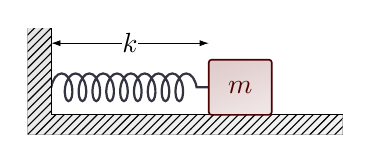
\begin{tikzpicture}
  \def\H{1.1}  % wall height
  \def\T{0.3}  % wall thickness
  \def\W{3.7}  % ground length
  \def\D{0.25} % ground depth
  \def\h{0.7}  % mass height
  \def\w{0.8}  % mass width
  \def\x{2.0}  % mass x position
  \def\y{1.22*\H} % x axis y position
  
  % AXIS
  \draw[ell] (0,1.3*\h) --++ (\x,0) node[midway,fill=white,inner sep=0] {$k$};
  
  % SPRING & MASS
  \draw[spring] (0,\h/2) --++ (\x,0);
  \draw[ground] (0,0) |-++ (-\T,\H) |-++ (\T+\W,-\H-\D) -- (\W,0) -- cycle;
  \draw (0,\H) -- (0,0) -- (\W,0);
  \draw[mass] (\x,0) rectangle++ (\w,\h) node[midway] {$m$};
  
\end{tikzpicture}
\end{figure}

The equation of motion of the system is $$m\frac{d^2q}{dt^2}=-kq,$$ where $q$ is the displacement.
And the analytical solution would be of the form $q=A\sin(\omega_0t+\phi),$ where $\omega=\frac{k}{m}$ and $A, \phi$ depends on the initial condition, which dictates the amplitude and phase of the motion. 
For this case, we have 
$$
\mathbf{f}(X)=\begin{pmatrix}
    \mathbf{a}(X)\\
    \mathbf{v}(X)\\
\end{pmatrix}
$$

\begin{figure}[H] 
  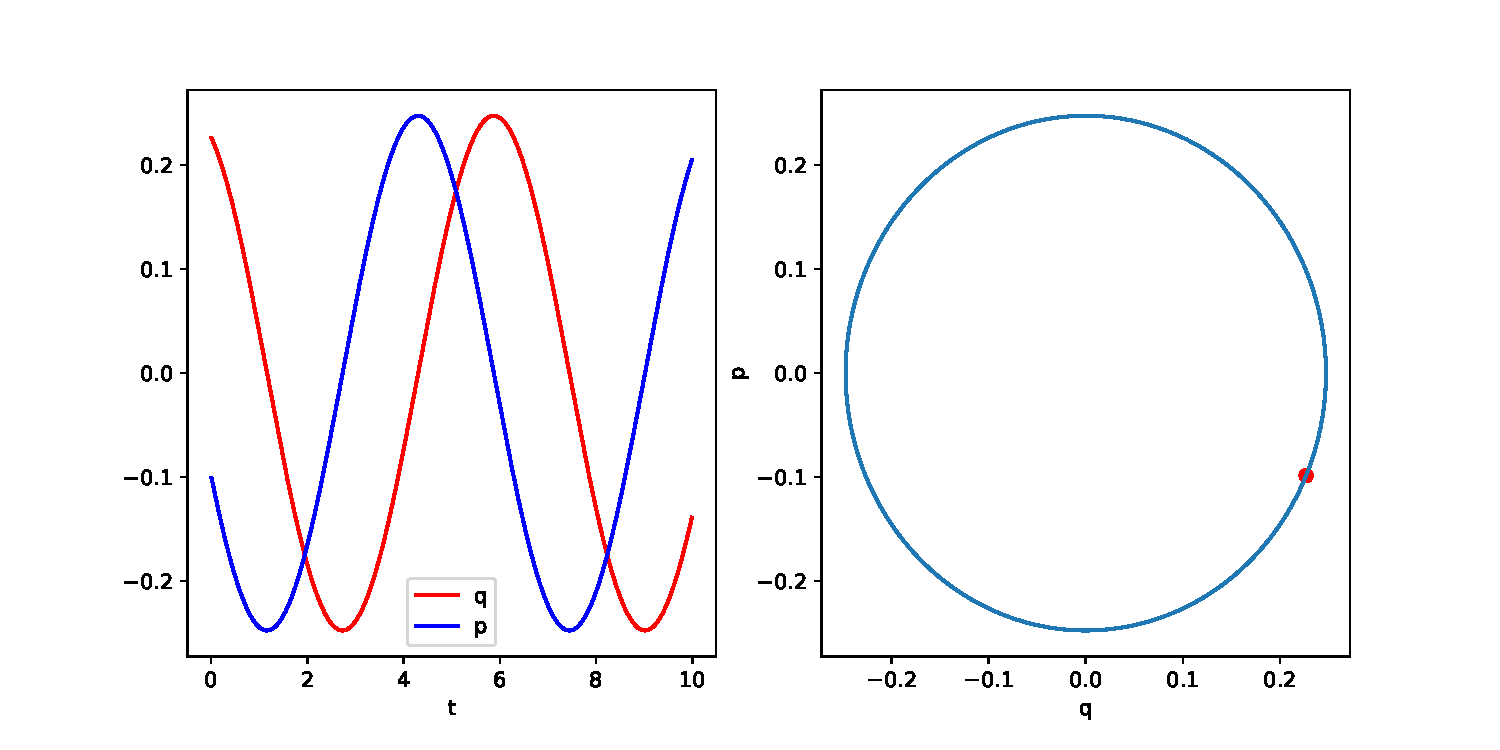
\includegraphics[width=0.6\linewidth]{../codes/figures/shm_trajectory_1D.pdf}
  \centering
  \caption{Example trajectory of SHM}
  \label{fig:shm_trajectory}
\end{figure}

We also have the energy, $E=\frac{mp^2}{2}+\frac{kq^2}{2},$
Therefore, to obtain our invariance $L$, we use the conservation of energy $\frac{dE}{dt}=0$ so we finally have $$L(a, v)=mpa+kqv=0$$
While $L$ is not able to be into a matrix form, it is a linear operator as shown below. 
If we have $$X_L\equiv\begin{pmatrix}
    \mathbf{x}_{L,1}\\
    \vdots\\
    \mathbf{x}_{L,\ell}\\
\end{pmatrix}=\begin{pmatrix}
    q_{L,1} & p_{L,1}\\
    \vdots & \vdots \\
    q_{L,\ell} & p_{L,\ell}\\
\end{pmatrix}\equiv\begin{pmatrix}
    \vdots & \vdots\\
    q_L & p_L\\
    \vdots & \vdots\\
\end{pmatrix},$$
then we have 
$$
L([\mathbf{f}(X_L)]) = \begin{pmatrix}
   mp_{L,1}a(q_{L,1},p_{L,1}) + kq_{L,1}v(q_{L,1},p_{L,1})\\ 
   \vdots \\
   mp_{L,\ell}a(q_{L,\ell},p_{L,\ell}) + kq_{L,\ell}v(q_{L,\ell},p_{L,\ell})\\ 
\end{pmatrix},
$$
which can be readily checked to be linear.
Combine with original GP prior assumption, we have 
$$
\begin{pmatrix}
    \mathbf{f}(X)\\
    L([\mathbf{f}(X_L)])\\
\end{pmatrix}
\sim\mathcal{N}
\left(\begin{pmatrix}
    0_{2n}\\0_{\ell}
\end{pmatrix},\begin{pmatrix}
   A & B \\
   C & D\\ 
\end{pmatrix}\right),
$$
where
$$
A=K(X,X), B=\begin{pmatrix}
    K_{RBF,a} \\ K_{RBF,v} \\
\end{pmatrix}\odot \begin{pmatrix}
    mP_L \\ kQ_L
\end{pmatrix}, C=B^T, D=K_{RBF,a}\odot m^2(p_L\otimes p_L) + K_{RBF,v}\odot k^2(q_L\otimes q_L),
$$
where $\odot$ is the elementwise product and $\otimes$ is the Kronecker product so that 
$$
P_L=\begin{pmatrix}
  p_{L,1}  & \dots & p_{L,\ell}  \\
  \vdots & \text{repeats n rows} &  \vdots\\
  p_{L,1}  & \dots & p_{L,\ell}  \\
\end{pmatrix},
Q_L=\begin{pmatrix}
  q_{L,1}  & \dots & q_{L,\ell}  \\
  \vdots & \text{reqeats n rows} &  \vdots\\
  q_{L,1}  & \dots & q_{L,\ell}  \\
\end{pmatrix}
$$
and we have 
$$
p_L\otimes p_L=\begin{pmatrix}
  p_{L,1}^2 & p_{L,1}p_{L,2} & \dots & p_{L,1}p_{L,\ell} \\
  \vdots & \vdots & \vdots & \vdots \\
  p_{L,\ell}p_{L,1} & p_{L,\ell}p_{L,2} & \dots & p_{L,\ell}^2 \\
\end{pmatrix},
q_L\otimes q_L=\begin{pmatrix}
  q_{L,1}^2 & q_{L,1}q_{L,2} & \dots & q_{L,1}q_{L,\ell} \\
  \vdots & \vdots & \vdots & \vdots \\
  q_{L,\ell}q_{L,1} & q_{L,\ell}q_{L,2} & \dots & q_{L,\ell}^2 \\
\end{pmatrix},
$$ 
These matrix expressions are derived as follows bt computing the covariance manually. 
For $B$, we wish to calculate 

\begin{align*}
B_{ij} &= \mathrm{Cov}(\mathbf{f}(X), L[\mathbf{f}(X_L)])_{ij} \\
       &= \mathrm{Cov}(\mathbf{f}(X)_i, L\mathbf{f}(X_L)_j) \\ 
       &= \begin{cases}
        \mathrm{Cov}(a(q_i, p_i), mp_{L,j}a(q_{L,j},p_{L,j}) + kq_{L,j}v(q_{L,j},p_{L,j})) & i\le n \\ 
        \mathrm{Cov}(v(q_i, p_i), mp_{L,j}a(q_{L,j},p_{L,j}) + kq_{L,j}v(q_{L,j},p_{L,j})) & i>n \\ 
       \end{cases} \\
       &= \begin{cases}
        K_{RBF,a}(\mathbf{x}_i, \mathbf{x}_{L,j}) mp_{L,j} & i\le n \\ 
        K_{RBF,v}(\mathbf{x}_i, \mathbf{x}_{L,j}) kq_{L,j} & i>n \\ 
       \end{cases}, \\
\end{align*}
and hence we have the form above. 
For $D$, we have
\begin{align*}
D_{ij} &= \mathrm{Cov}(L[\mathbf{f}(X_L)], L[\mathbf{f}(X_L)])_{ij} \\
       &= \mathrm{Cov}(mp_{L,i}a(q_{L,i},p_{L,i}) + kq_{L,i}v(q_{L,i},p_{L,i}), mp_{L,i}a(q_{L,i},p_{L,i}) + kq_{L,i}v(q_{L,i},p_{L,i})) \\
       &= m^2p_{L,i}p_{L,j}K_{RBF,a}(\mathbf{x}_{L,i},\mathbf{x}_{L,j}) + k^2q_{L,i}q_{L,j}K_{RBF,v}(\mathbf{x}_{L,i},\mathbf{x}_{L,j})
\end{align*}
using the bilnear property of the covariance operator and the fact that $v$ and $a$ are independent.
Since we assume invariance on these invariance points, we will condition on $L([\mathbf{f}(X_L)])=0.$
Now we can simply use the Gaussian conditional formula to obtain the Schur Complement using equation \ref{equ:normal_condtion}.
$$
\mathbf{f}(X)|L[\mathbf{f}(X_L)]=0\sim\mathcal{N}(0_{2n},A-BD^{-1}C),
$$
we will then call the resulting covariance our Invariance Kernel for 1D SHM, $K_L$.

\subsection{Non Linear}
The idea is pretty much the same for nonlinear system compared to linear; however, the fitting is expected to be more difficult.
A simple nonlinear system in every day life is a simple pendulum as shown in figure below.
The governing equation is 
$$
\frac{d^2q}{dt^2}=-\frac{g}{\ell}\sin q, 
$$
where $q$ is the angle of displacement this time and we have example trajectory in \ref{fig:pendulum_trajectory}, where we can see the effect of nonlinearity on the shape. 
The nonlinear dynamics arises from the sine term above, which will complicate the derivation for invariance kernel slightly. 
However, since $\sin x \approx x$ at small angle, this system is approximately linear under small displacement. 
There is no analytical solution to this nonlinear problem in general, besides the small displacement case, which will be 1D SHM.

\begin{figure}[H] 
  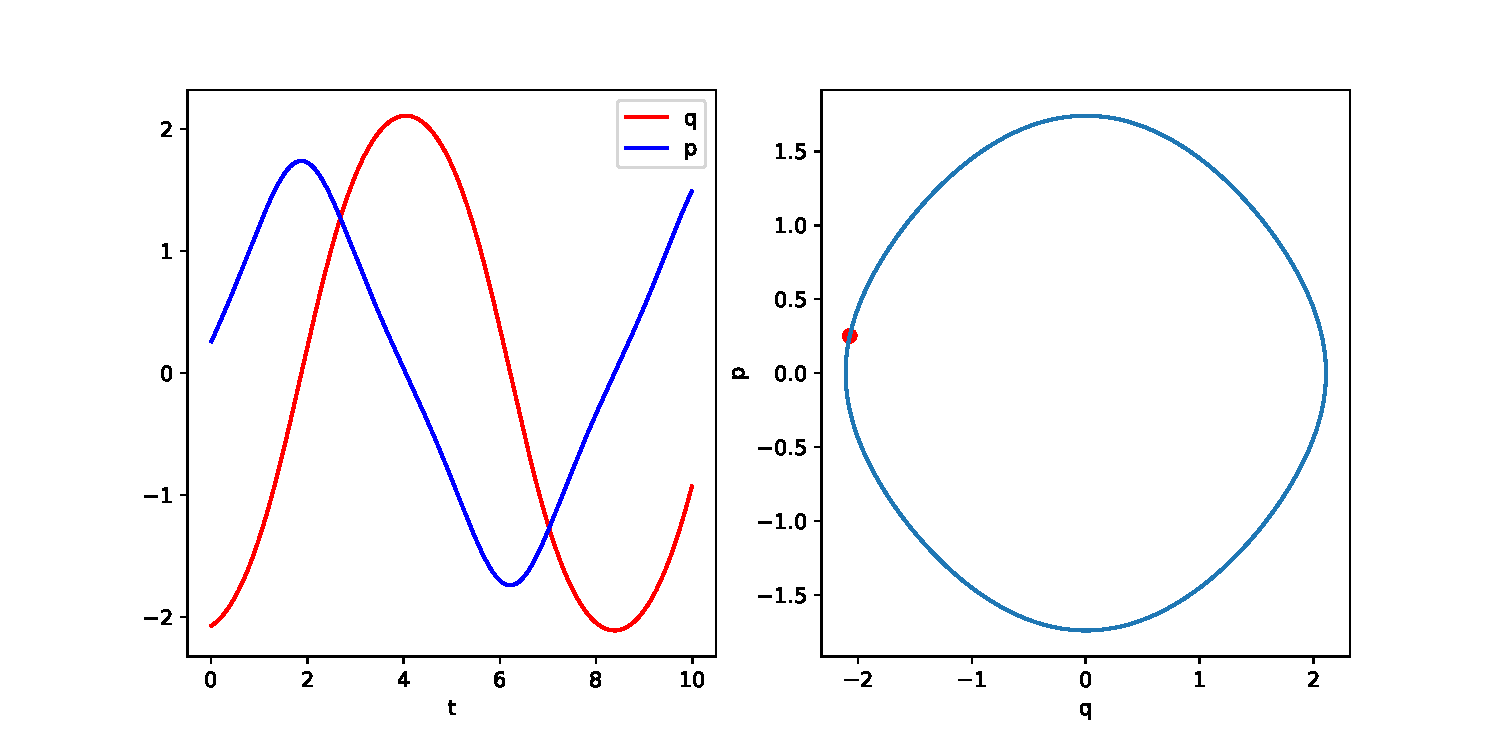
\includegraphics[width=0.6\linewidth]{../codes/figures/pendulum_trajectory_1D.pdf}
  \centering
  \caption{Example trajectory of pendulum}
  \label{fig:pendulum_trajectory}
\end{figure}

This time we have energy, $E=\frac{m\ell^2p^2}{2}+mg\ell(1-\cos q)$, and by setting the time derivative to 0, we have 
$$L(a, v)=\frac{dE}{dt}=m\ell^2pa+mg\ell(\sin q)v=0.$$
If we cancel out the common term $m\ell$ since their product cannot be zero, we have $$L(a,v)=\ell pa+g(\sin q)v=0$$
Most of the terms are unchanged from the linear case. 
However, this time, 
$$
B=\begin{pmatrix}
    K_{RBF,a} \\ K_{RBF,v} \\
\end{pmatrix}\odot \begin{pmatrix}
    \ell P_L \\ g\sin(Q_L)
\end{pmatrix}, D=K_{RBF,a}\odot \ell^2(p_L\otimes p_L) + K_{RBF,v}\odot g^2(\sin(q_L)\otimes \sin(q_L)),
$$
where 
$$
\sin(Q_L) = g\begin{pmatrix}
  \sin(q_{L,1})  & \dots & \sin(q_{L,\ell})  \\
  \vdots & \text{reqeats n rows} &  \vdots\\
  \sin(q_{L,1})  & \dots & \sin(q_{L,\ell})  \\
\end{pmatrix},
$$
$$
\sin(q_L)\otimes \sin(q_L)=\begin{pmatrix}
  \sin(q_{L,1})^2 & \sin(q_{L,1})\sin(q_{L,2}) & \dots & \sin(q_{L,1})\sin(q_{L,\ell}) \\
  \vdots & \vdots & \vdots & \vdots \\
  \sin(q_{L,\ell})\sin(q_{L,1}) & \sin(q_{L,\ell})\sin(q_{L,2}) & \dots & \sin(q_{L,\ell})^2 \\
\end{pmatrix},
$$
derived in exactly the same way as the linear case. 

\begin{figure}[H]
     \centering
     \begin{subfigure}[b]{0.5\linewidth}
        \centering
        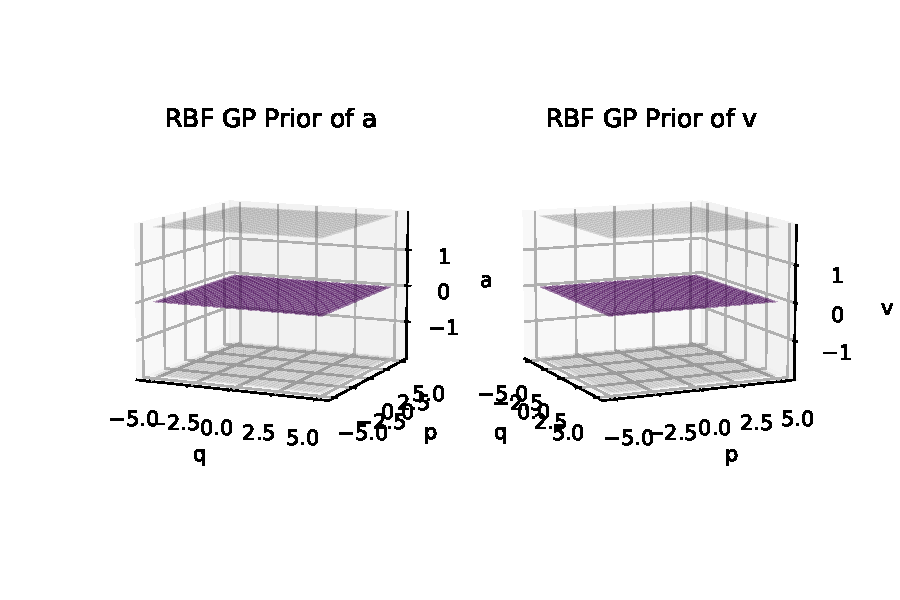
\includegraphics[width=\linewidth]{../codes/figures/prior_shm_rbf.pdf}
        \caption{RBF prior}
        \label{fig:prior_shm_rbf}
     \end{subfigure}
     \hfill
     \begin{subfigure}[b]{0.5\linewidth}
         \centering
         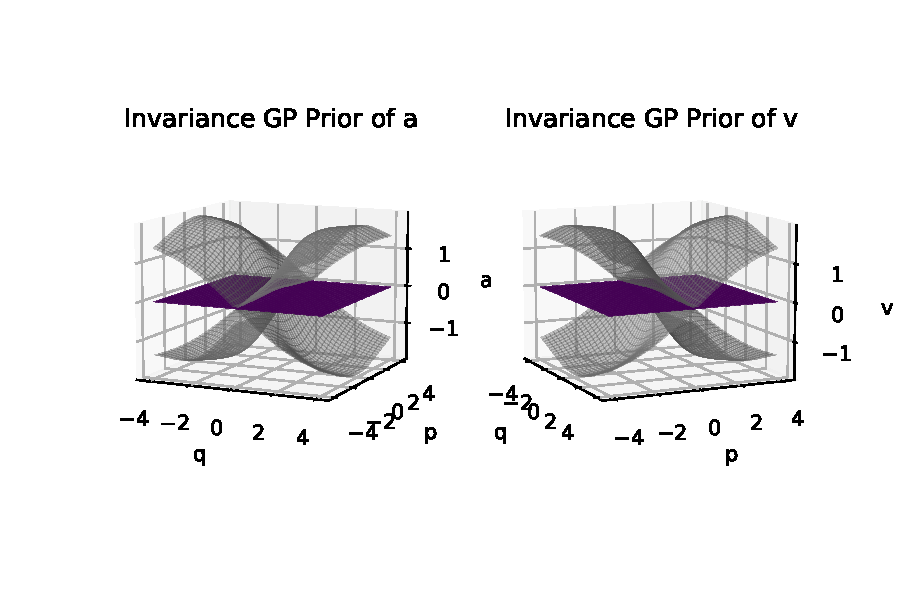
\includegraphics[width=\linewidth]{../codes/figures/prior_shm_invariance.pdf}
         \caption{SHM invariance prior}
         \label{fig:prior_shm_invariance}
     \end{subfigure}
     \hfill
     \begin{subfigure}[b]{0.5\linewidth}
         \centering
         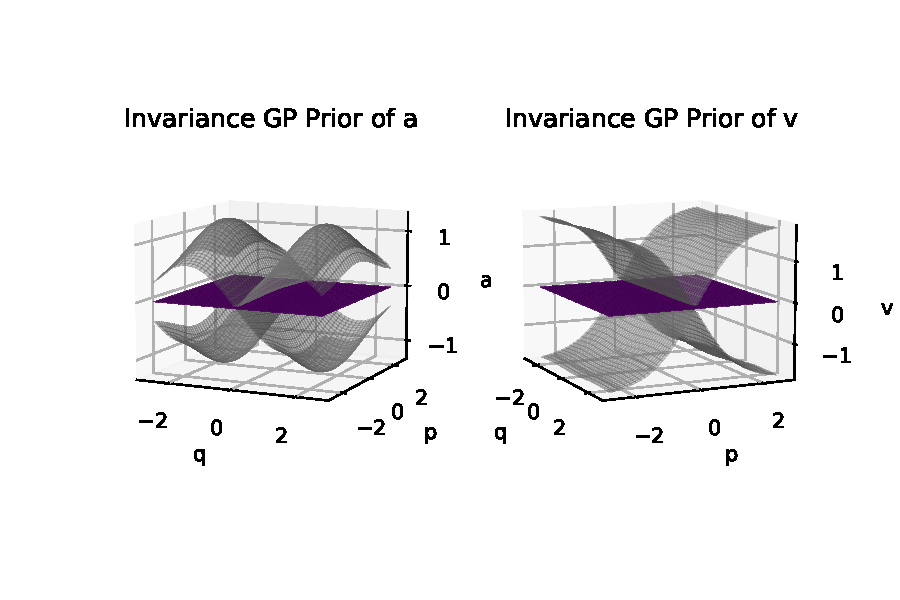
\includegraphics[width=\linewidth]{../codes/figures/prior_pendulum_invariance.pdf}
         \caption{Pendulum invariance prior}
         \label{fig:prior_pendulum_invariance}
     \end{subfigure}
        \caption{Priors}
        \label{fig:priors}
\end{figure}

\section{Damped System}
In previous sections, we have considered a perfect system, i.e. ideal world without frictions and the conservation of energy is completely obeyed such that $L=0$ exactly.
However, in a real system, there will be dissipation where energy is lost in the form of heat etc.  
Therefore, to model that, we need to allow "approximate" invariance, such that the invariance $L$ is noisy and not always equal to zero, i.e. soft invariance.
To account for that, in a similar spirit to when we add noise to the underlying latent GP to represent noise signal in equation, where we have $K+\sigma_n^2 \mathbb{I}$;
Here, since the white noise is uncorrelated, the only place the noise will enter is $D$, so we simply have to add a noise term to $D$ and replace all $D$ with $\tilde{D}=D+\epsilon \mathbb{I}$, where $\epsilon$ is a parameter to be learnt. 
For the data, we will model the system as a damped SHM or pendulum with linear velocity dependent force.
If we denote $\omega_0^2=k/m$ or $\omega_0^2=g/\ell$
We will have the equation of motion for SHM and pendulum respectively
$$
\frac{d^2q}{dt^2}+2\gamma\frac{dq}{dt}+\omega_0^2q=0; \frac{d^2q}{dt^2}+2\gamma\frac{dq}{dt}+\omega_0^2\sin q=0 ,
$$
and the $\gamma$ is the damping factor that controls how much frictional force there is. 
Note that we will only focus on underdamping case ($\gamma < \omega_0^2$)so that the system still oscillate but with gradually reduced amplitude instead of critical damped ($\gamma=\omega_0^2$) or overdamped ($\gamma>\omega_0^2$) case where the system simply slowly decays to still.
An example trajectory for damped SHM and damped pendulum is shown below in figure \ref{fig:damped_trajectory}.

\begin{figure}[H]
     \centering
     \begin{subfigure}[b]{\linewidth}
        \centering
        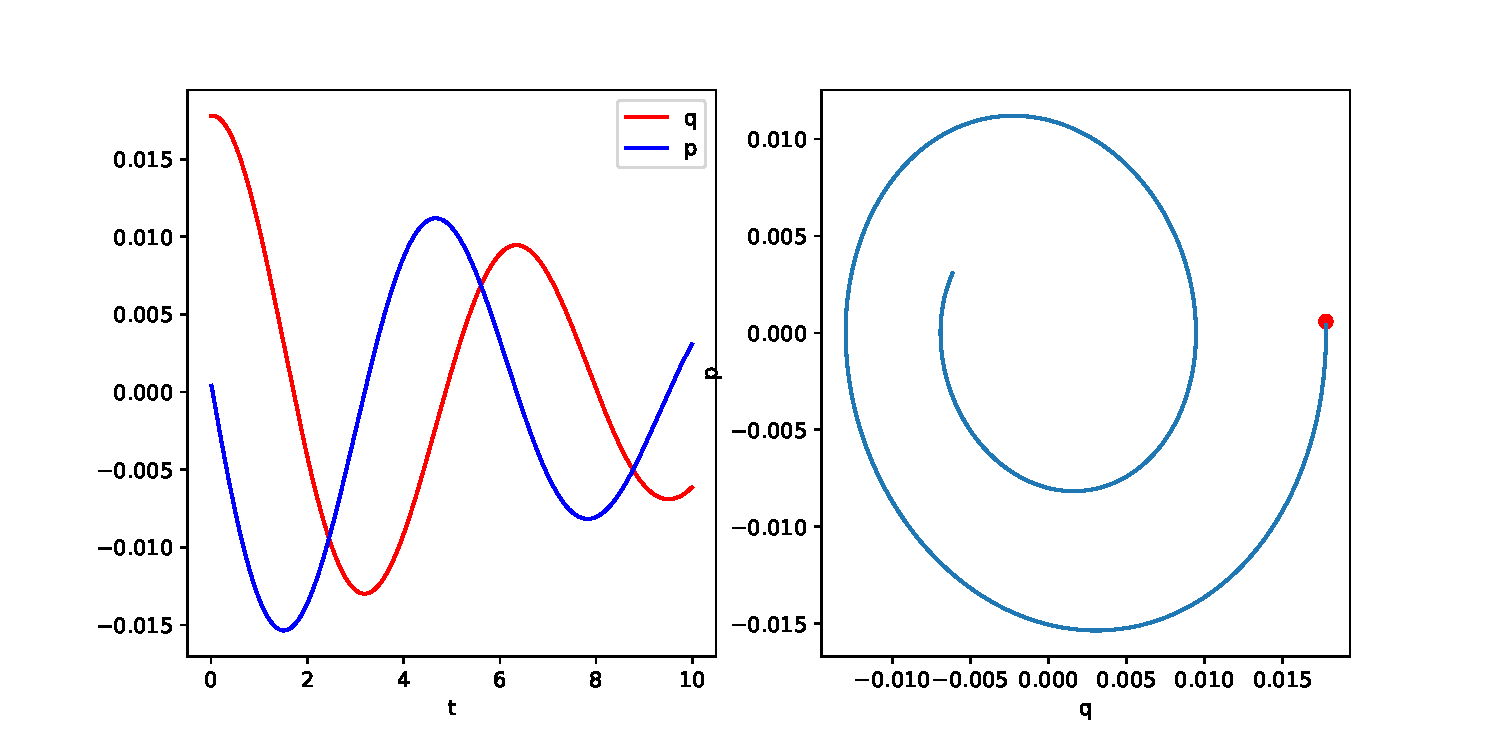
\includegraphics[width=0.5\linewidth]{../codes/figures/damped_shm_trajectory_1D.pdf}
        \caption{Example trajectory of damped SHM}
        \label{fig:damped_shm_trajectory}
     \end{subfigure}
     \hfill
     \begin{subfigure}[b]{\linewidth}
        \centering
        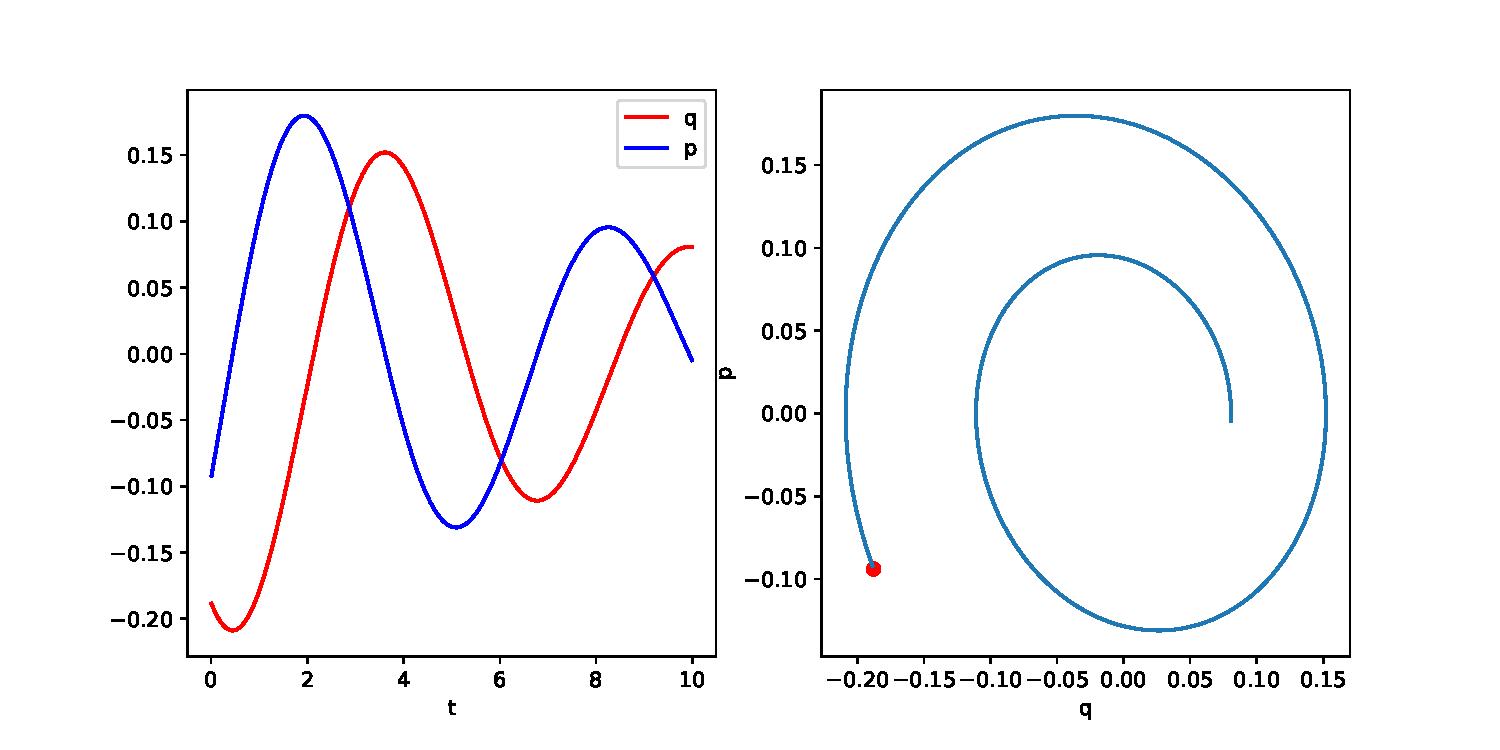
\includegraphics[width=0.5\linewidth]{../codes/figures/damped_pendulum_trajectory_1D.pdf}
        \caption{Example trajectory of damped pendulum}
        \label{fig:damped_pendulum_trajectory}
     \end{subfigure}
        \caption{Example trajectories of damped systmes}
        \label{fig:damped_trajectory}
\end{figure}

\section{2D System}
A 2D system is not that different from an 1D system. The major difference being there will be two more variables. 
We will again look at two simple examples, a linear 2D SHM, and a nonlinear double pendulum.
\subsection{Linear}
A simple extension to 1D SHM to 2D is just allowing the spring to be at an angle so that the system is now in a 2D space.
Again, the equations are simple that we have two equations for the two coordinates.
$$
\begin{cases}
    \frac{d^2{q_1}}{dt^2} = -\frac{k}{m}q_1\\
    \frac{d^2{q_2}}{dt^2} = -\frac{k}{m}q_2\\
\end{cases}
$$
The analytical solution is exactly the same, but now there are two of them with differing amplitudes and phases depending on the initial condition. 
And now we have $$\mathbf{f}(X)=\begin{pmatrix}
    \mathbf{a_1}(X)\\
    \mathbf{a_2}(X)\\
    \mathbf{v_1}(X)\\
    \mathbf{v_2}(X)\\
\end{pmatrix},$$
where $\mathbf{a_1}$ and $\mathbf{a_2}$ are the dynamics or time derivative for $\mathbf{p_1}$ and $\mathbf{p_2}$ respectively; similarly $\mathbf{v_1}$ and $\mathbf{v_2}$ are the time derivative of $\mathbf{q_1}$ and $\mathbf{q_2}$.
In this system, the energy is the sum of energy in the two directions so $E=\frac{m(p_1^2+p_2^2)}{2}+\frac{k(q_1^2+q_2^2)}{2}$ and so the invariance $L(a_1, a_2, v_1, v_2)=\frac{dE}{dt}=mp_1a_1+mp_2a_2+kq_1v_1+kq_2v_2=0.$
Now our naive baseline GP has the kernel
$$
K(X,X')=\begin{pmatrix}
K_{RBF,a_1}(X,X') & 0 & 0 & 0 \\
0 & K_{RBF,a_2}(X,X') & 0 & 0 \\
0 & 0 & K_{RBF,v_1}(X,X') & 0 \\
0 & 0 & 0 & K_{RBF,v_2}(X,X') \\
\end{pmatrix}.
$$
We will then have the joint distribution of
$$
\begin{pmatrix}
    \mathbf{f}(X)\\L[\mathbf{f}(X_L)]\\
\end{pmatrix}
\sim\mathcal{N}
\left(
\begin{pmatrix}
    0_{4n} \\ 0_{\ell}
\end{pmatrix},
\begin{pmatrix}
    A & B \\
    C & D\\
\end{pmatrix}
\right),
$$
with 

$$
A=K(X, X'), 
B=\begin{pmatrix}
    K_{RBF, a_1}\\
    K_{RBF, a_2}\\
    K_{RBF, v_1}\\
    K_{RBF, v_2}\\
\end{pmatrix}\odot
\begin{pmatrix}
mP_{1L}  \\
mP_{2L}  \\
kQ_{1L}  \\
kQ_{2L}  \\
\end{pmatrix},
C=B^T 
$$

\begin{gather*}
D=K_{RBF,a_1}m^2\odot(p_{1L}\otimes p_{1L}) + K_{RBF,a_2}m^2\odot(p_{2L}\otimes p_{2L})\\+K_{RBF,v_1}k^2\odot(q_{1L}\otimes q_{1L})+K_{RBF,v_2}k^2\odot(q_{2L}\otimes p_{2L})
\end{gather*}

where the terms are defined the exact same way as before, but now with respect to different coordinates, and the derivation are also the same.
We will then again take the Schur Complement.
\subsection{Non Linear}
Now we will to introduce double pendulum, which is a fairly nonlinear system and quite complicated. 
It has two mass blobs $m_1$ and $m_2$ as well as two lengths for the pendlum stem $\ell_1$ and $\ell_2$.
The defining equations are as follows:
$$
\begin{cases}
\frac{d^2q_1}{dt^2}=\frac{-g\left(2 m_{1}+m_{2}\right) \sin q_1-m_{2} g \sin \left(q_1-2 q_2\right)-2 \sin \left(q_1-q_2\right) m_{2}\left(p_2^{2} l_{2}+p_1^{2} l_{1} \cos \left(q_1-q_2\right)\right)}{l_{1}\left(2 m_{1}+m_{2}-m_{2} \cos \left(2 q_1-2 q_2\right)\right)} \\
\frac{d^2q_2}{dt^2}=\frac{2 \sin \left(q_1-q_2\right)\left(p_1^{2} l_{1}\left(m_{1}+m_{2}\right)+g\left(m_{1}+m_{2}\right) \cos q_1+p_2{ }^{2} l_{2} m_{2} \cos \left(q_1-q_2\right)\right)}{l_{2}\left(2 m_{1}+m_{2}-m_{2} \cos \left(2 q_1-2 q_2\right)\right)}
\end{cases}
$$
As we can see, it is very complicated in term of the form.
We also have form of energy 
$$
E = -(m_1+m_2)gl_1\cos q_1-m_2gl_2\cos q_2+ \frac{m_1l^2_1p_1^2}{2}+\frac{m_2}{2}(l^2_1p_1^2+l^2_2p_2^2+2l_1l_2p_1p_2\cos(q_1-q_2))
$$
While the form is more complicated, the underlying principle to construct the invariance kernel. 
We again differentiate with respect to time and set it to zero to obtain the invariance equation to obtain 
\begin{gather*}
L(a_1, a_2, v_1, v_2)=\frac{dE}{dt} = (m_1+m_2)gl_1\sin\theta_1v_1+m_2gl_2\sin\theta_2v_2+m_1l_1^2\dot{\theta}_1a_1+\\m_2(l_1^2\dot{\theta}_1a_1+l_2^2\dot{\theta}_2a_2+l_1l_2(\dot{\theta}_2\cos(\theta_1-\theta_2)a_1+\dot{\theta}_1\cos(\theta_1-\theta_2)a_2-\dot{\theta_1}\dot{\theta_2}\sin(\theta_1-\theta_2)(v_1-v_2)))=0
\end{gather*}
The form of the invariance matrix is too cubersome to write down, but the derivation is as straightforward as before. 



\section{Learning Invariance}
Previously, we have assumed the knowledge of the dynamics equation from Newton's Law, which allowed us to derive the energy and thereafter the invariance equation. 
However, for the kernel to be useful in real life, we cannot assume the equations of the system beforehand, since if we have the knowledge, then the system is pretty much solved that we can just use an ODE integrator to obtain the trajectories. 
Therefore, we should find a way for the system to learn the form of invariance from data directly.
One way to do so is to parameterise our invariance function and allow the system to learn the coefficients by maximising the log marginal likelihood.
\subsection{1D system}
A simple way to parameterise an unknown function, when the problem is relatively bounded is to use polynomial basis to paramertise the unknown function $L(a,v)$.
In 1D cases, for our examples, they are simple enough so that $L(a,v)$ is a sum of a function of $a$ and $p$ only, $f_pa$ and a different function of $v$ and $q$ only, $g_q(v)$ so that $L(a,v)=f_p(a)+g_q(v)$.
In the 1D SHM case, $f_p(a)=mpa$ and $g_q(v)=kqv$.
For simple pendulum, we have $f_p(a)=\ell pa$ and $g_q(v)=\sin qv$.
We will therefore set $$f_p(a)=\sum_{i=0}^{n_f}c_{f,i}p^i,g_q(a)=\sum_{i=0}^{n_g}c_{g,i}q^i,$$
where $c_{f,i}, c_{g,i}$ are the parameter we will optimise based on marginal likelihood and we will evaluate different degree of polynomial $n_f, n_g$ and see which gives the best results. 

\subsection{2D system}
In 2D, things are a bit more complicated. For example, it is very clear that in double pendulum, the invariance function is not seperable.
Instead, we need to consider all combinations of polynomials; i.e. multivariate polynomial.
Therefore, for 2D we have $L(a,v)=f_1a_1+f_2a_2+g_1v_1+g_2v_2.$
We will paramertise each of $f_1, f_2, g_1, g_2$ with $$\sum_{i,j,k,l=0}^{n}c_{ijkl}p_1^ip_2^jq_1^kq_2^l$$
Therefore, there will be many more coefficients.

\chapter{Experiments}
\section{Data Generation}
To generate the data, we use a Runge-Kutta integrator to generate data using the equation of motions for each problem. 
We also added some small Gaussian noise $10^{-8}$ to the dynamics to reflect the real world better as well as stablising the integrator.
Since we aim to predict the value of dynamics at any point in the input space, we use the dynamics as targets , Y. 
This is done by combining forward and backward finite difference (midpoint method) to compute the gradient. 
We also choose the time step to be $0.01$ to ensure sufficient accuracy for the integrator.
For training data, X, we choose a few random starting point within a range (datails depends on the task as described later) in the input space and generate data from there for a number of timesteps (which is fixed at 10 points per trajectory in this report). 
To assess the performance, we generate the test set using the same input range, we will pick three different starting points and then average the result.
Without loss of generality, we choose $m=k=1$ and $g=\ell=1$ for 1D and 2D SHM and simple pendulum for simplicity of presentation. 
For the damping, we will choose $\gamma= 0.1$, which is fairly strongly damped as shown in figure \ref{fig:damped_pendulum_trajectory}, \ref{fig:damped_shm_trajectory}. 
For double pendulum, we also set $m_1=m_2=\ell_1=\ell_2=g=1.$

\section{Evaluation Method}
We will mainly use the mean squared error (MSE) between the trajectory prediction and ground truth as our evaluation metrics. 
We also illustrate the amount of energy (using the exact expression) along the trajectory to demonstrate that invariance is obeyed.
For learning the invariance in 1D case, we can also further compare the true invariance and the learnt invariance up to a multiplicative constant.
However, it is not possible to visualise in 2D cases so we will simply assess the conservation of energy (invariance) performance.

\section{Implementation Technicalities}
We will need to add jitter, a diagnoal matrix of small value, to the $LKL^T$ matrix in equation \ref{equ:invariance_condition}.
This is due to the fact that we need the invert it and it will be more stable numerically if we add a little bit of jitter in the range of $10^{-6}$ to $10^{-4}$, and its effect on the model will be explained in the sections below.
Similarly, for stability, when backpropagating to optimise the hyperparameters with respect to marginal likelihood, we need to narrow range of search such that the value is more reasonable.
It is particularly important in our dynamical systems since, for example, in SHM the equation of motion is $a=-q$ and $v=p$, so that is will be a 2D plane extends to infinity;
as a result, if the GP learns "correctly", the lengthscales of some directions will be very large or $\infty$, and that will be problematic and it would not affect the performance a lot if we limit the lengthscales for a much smaller value.
Therefore, here I would set the range of both lengthscales and variable to be around the twice to three times the maximum range possible.
For example, if we have maximum range of $\pm 3$, my upper bound for search is set to $10$ and lower bound is $10^{-3}$.
Another change we made in 2D SHM is to scale the data using MinMax scaler to squash them to be between $\pm 1$. 
This is done since the polynomial behaves better around this region.

\subsection*{Invariance points $X_L$}
In low dimensions, we could simply allow $X_L$ to be a evenly spaced grid in the input space, and we will call the number of points in each dimension the \textbf{invariance density}.
So that if I have an invariance density of $40$, it means my $X_L$ will contain $1600$ points. 
However, conditioning on a grid of invariance points is simply not scalable in high dimensions. 
If we have an invariance density of 10 in a $\pm 5$ range for 2D SHM (spacing of 1), then we will have 10000 points. 
We can easily run out of memory and also taking the matrix inverse are very difficult and time consuming.
As a result, to make the approach scalable to high dimensional space, we will use the idea of local invariance. 
The idea is straightforward, we simply sample uniformly (30-80 points) in the local region around the training and testing points and set them as $X_L$ (we choose a torus shape around the data points so that we will not have invariance points too close to the data points, which will be unstable).
Note that we only sampled once, so that the same local grid will be centred on every training and testing points; this is done to remove the randomness for stability and dependence on the data.
This works on the assumption that only the region around testing points will be the most important to predict in terms of conditioning; and to use the same kernel, we also have to condition on the region around training points, which is also important to help maximising the marginal likelihood objective when we are learning the invariance function.
Another evidence that supports the use of local invariance, which have much fewer points than using a grid, is demonstrated below where we show that there is a diminishing return in increasing the number of invariance points so that actually not that many invariance points is needed to achieve a good performance. 

\section{SHM}
We start with the 1D SHM case, and for the data we will have only one trajectory starting randomly in $-3\le q\le3$ and $p$ to be between $\pm 0.3$.
We chose $p$ to be smaller so that the future trajectory does not overshoot the upper bound of $q$ too much. 
We allow the integrator to run for $0.1$ seconds so there will be in total 10 training points (10 time steps). 
We will then draw three test points from the same range as training, to assess the performance of the predictive power for 3 seconds (300 points) and average the MSE over the three trajectories. 
In figure \ref{fig:shm_prediction}, \ref{fig:damped_shm_energy}, we have chosen one trajectory at random to illustate the predictions as well as the energy along the trajectory.
For this task, we have used a jitter amount of $10^{-5}$ and an invariance density of 20 between $\pm 3$ in both $p$ and $q$ direction.
We have also plotted the posterior distribution of using invariance kernel and compare that to using naive RBF kernel in figure \ref{fig:posterior_shm}.
We can see the invariance has much better predictive power and generalisability.
For learning the invariance, we test all combinations of polynomials of $f(p)$ and $g(q)$, each with degree 0, 1, 2, 3 (i.e. up to cubic term) so there will be 16 of them to optimise, and we choose the pair with the highest marginal likelihood. 
We initialise the coefficients with normal distribution with variance of $10^{-3}$, we also restrict the search space to be between $\pm 1$.
We have also added a Laplace prior on the coefficients with variance 0.1 since we expect most coefficients would be zero and Laplace prior encourage sparse solution.
The learnt $f(p)$ and $g(q)$ is plotted in figure \ref{fig:shm_learnt}.
The performance is summarised in table \ref{tab:shm_performance}.

\begin{table}[H]
  \centering
  \begin{tabular}{l l l l }
\hline
Method           & RBF & Known Invariance&  Learnt Invariance\\
  \hline
Log Marginal Likelihood & 74.66 & 86.28 & 83.32  \\
MSE & 3.5563 & 0.1057 & 0.0927 \\
                    \hline
  \end{tabular}
  \caption{SHM performance}
  \label{tab:shm_performance}
\end{table}

\begin{figure}[H]
        \centering
        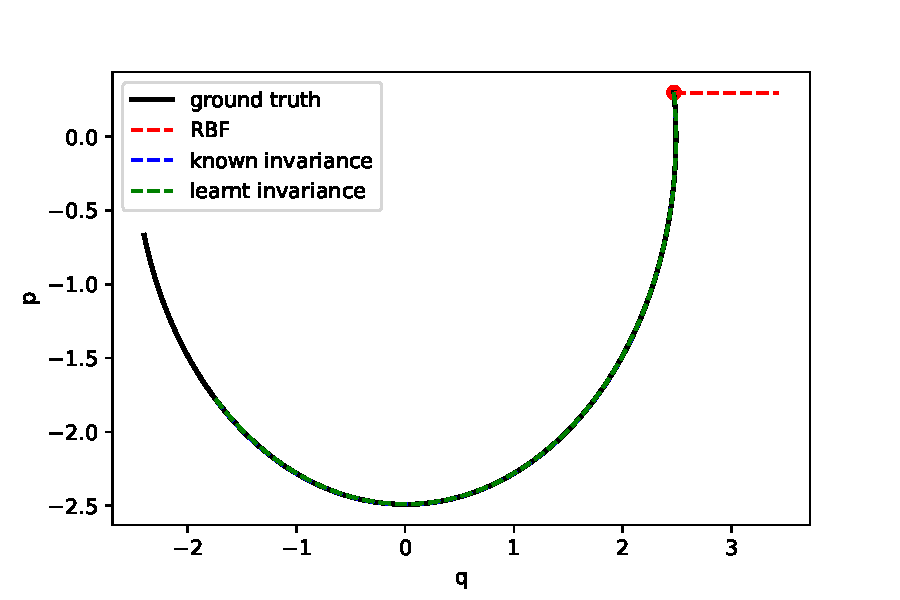
\includegraphics[width=0.8\linewidth]{../codes/figures/shm_predicted.pdf}
        \caption{SHM predicted trajectory}
        \label{fig:shm_prediction}
\end{figure}

\begin{figure}[H] 
  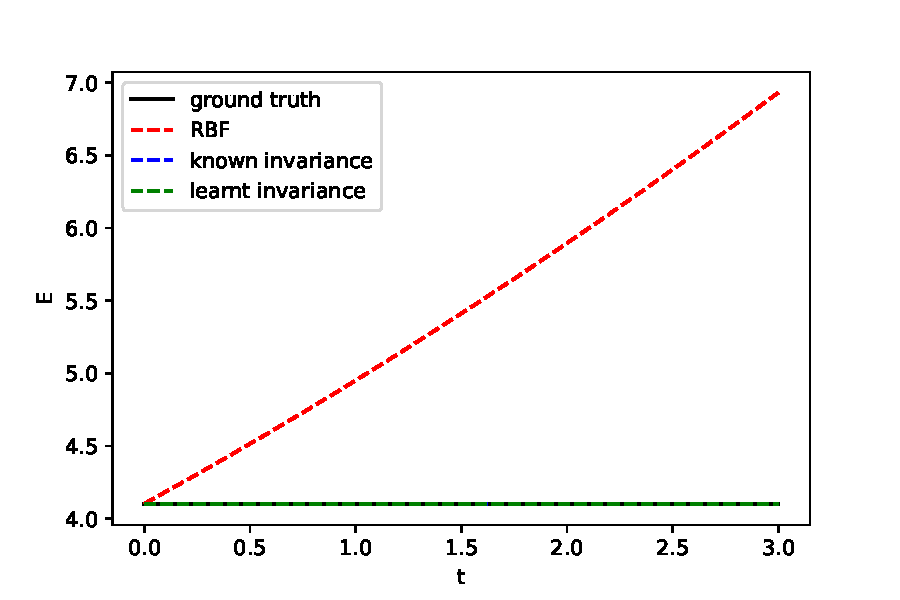
\includegraphics[width=0.8\linewidth]{../codes/figures/shm_energy.pdf}
  \centering
  \caption{Energy conservation for SHM}
  \label{fig:shm_energy}
\end{figure}

\begin{figure}[H] 
  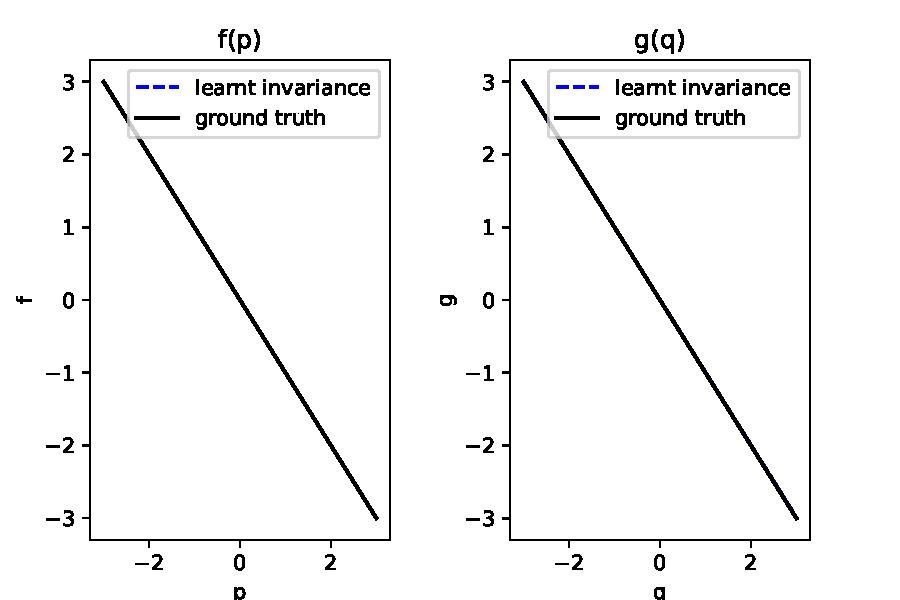
\includegraphics[width=0.8\linewidth]{../codes/figures/shm_learnt.pdf}
  \centering
  \caption{Learnt invariance for SHM}
  \label{fig:shm_learnt}
\end{figure}

\begin{figure}[H]
     \centering
     \begin{subfigure}[b]{\linewidth}
        \centering
        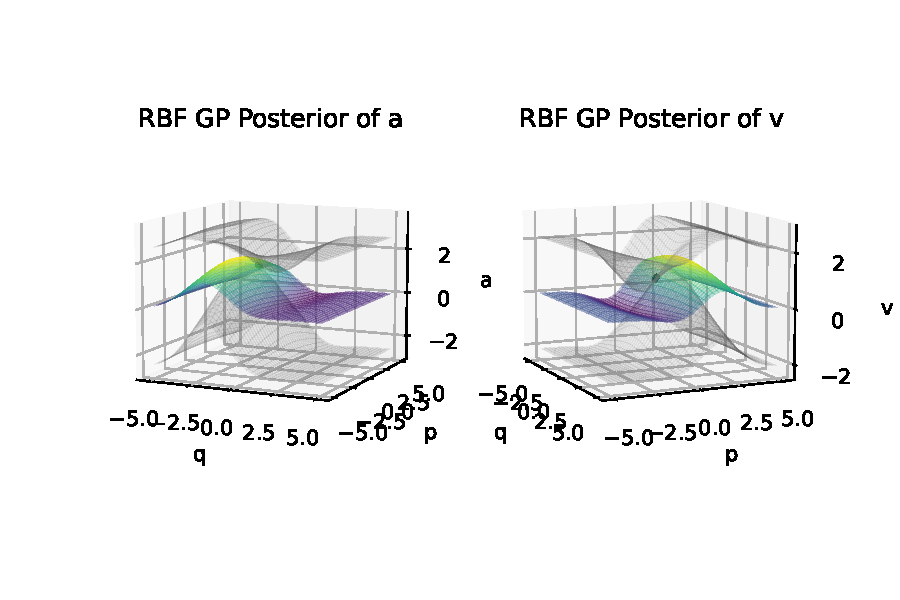
\includegraphics[width=\linewidth]{../codes/figures/posterior_shm_rbf.pdf}
        \caption{SHM RBF posterior}
        \label{fig:posterior_shm_rbf}
     \end{subfigure}
     \hfill
     \begin{subfigure}[b]{\linewidth}
         \centering
         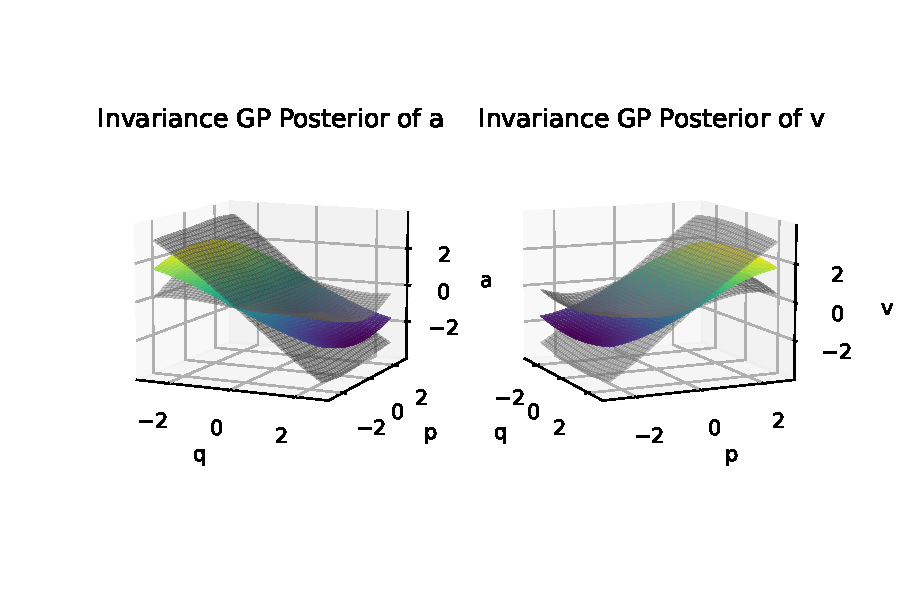
\includegraphics[width=\linewidth]{../codes/figures/posterior_shm_invariance.pdf}
         \caption{SHM invariance posterior}
         \label{fig:posterior_shm_invariance}
     \end{subfigure}
        \caption{SHM posteriors}
        \label{fig:posterior_shm}
\end{figure}



We can clearly see the naive RBF kernel failed to learn at all as it does not have enough example data to genealise, as we can see from \ref{fig:posterior_shm_rbf}, so that it is only able to predict well in the region where the data are. 
On the other hand, from \ref{fig:posterior_shm_invariance} and the prediction performance, we can see the invariance kernel has much better generalisation ability.
From the energy plot in figure \ref{fig:shm_energy}, we again see both the known and learnt invariance obeys the invariance very well while the RBF kernel does not at all.
In this case, the learnt invariance performs almost exactly as the known form, as we can also see in figure \ref{fig:shm_learnt}, and has successfully recovered the physics. 


\section{Pendulum}
In this task, the experiment setup is essentially exactly the same as the SHM case. 
However, since this time the dynamics is more complicated, we will draw three different starting points for training between $q=\pm 150^{\circ}$ and $\pm 10^{\circ}$ for $p$, so in total 30 points.
This time, since it is a harder task, we will use an invariance density of 30 between $\pm 150^{\circ}$.
We again have the prediction performance summarised in table \ref{tab:pendulum_performance} as well as figures \ref{fig:pendulum_prediction}, \ref{fig:pendulum_energy} and the posteriors in \ref{fig:posterior_pendulum}.
The learnt polynomial is in \ref{fig:pendulum_learnt}.

\begin{table}[H]
  \centering
  \begin{tabular}{ l l l l}
    \hline
Method           & RBF & Known Invariance&  Learnt Invariance\\
                    \hline
Log Marginal Likelihood & 233.89 & 262.59 & 255.76  \\
MSE & 0.0500 & 0.0025 & 0.0020 \\
    \hline
  \end{tabular}
  \caption{Pendulum performance}
  \label{tab:pendulum_performance}
\end{table}

\begin{figure}[H]
        \centering
        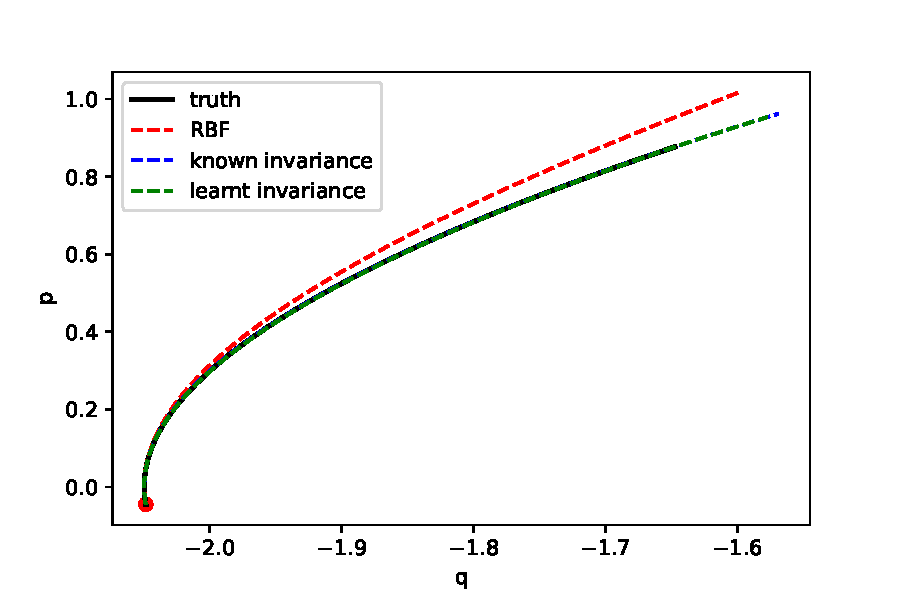
\includegraphics[width=0.8\linewidth]{../codes/figures/pendulum_predicted.pdf}
        \caption{pendulum predicted trajectory}
        \label{fig:pendulum_prediction}
\end{figure}

\begin{figure}[H] 
  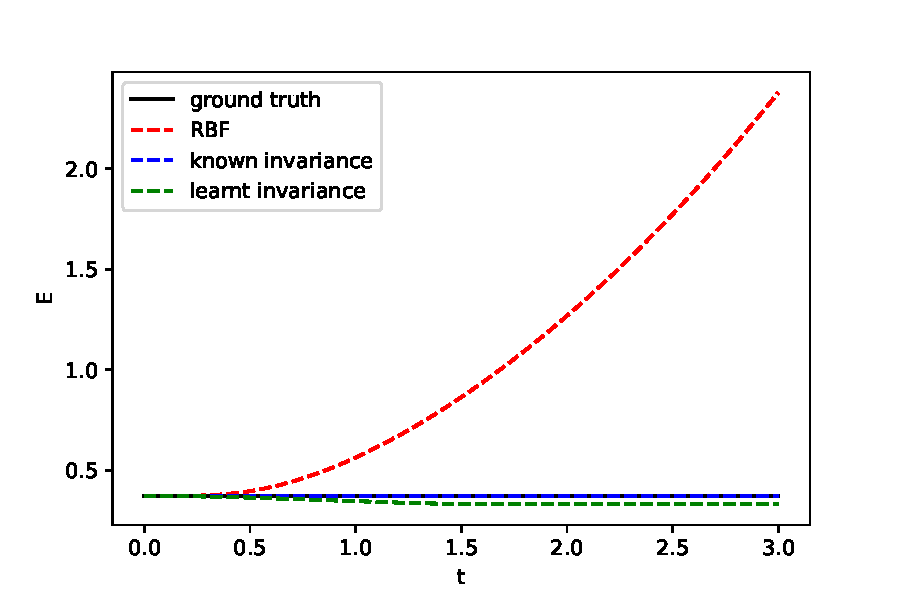
\includegraphics[width=0.8\linewidth]{../codes/figures/pendulum_energy.pdf}
  \centering
  \caption{Energy conservation for pendulum}
  \label{fig:pendulum_energy}
\end{figure}

\begin{figure}[H] 
  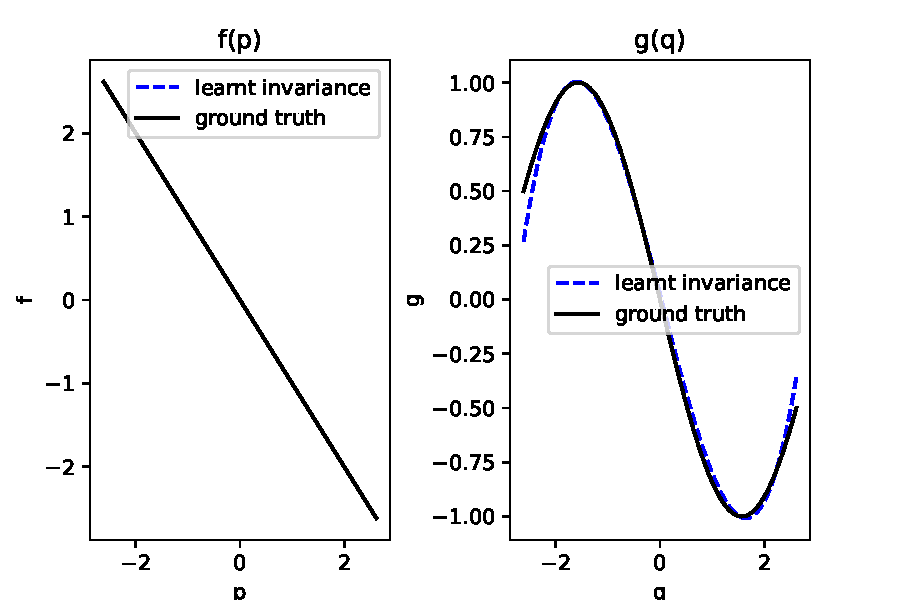
\includegraphics[width=0.8\linewidth]{../codes/figures/pendulum_learnt.pdf}
  \centering
  \caption{Learnt invariance for pendulum}
  \label{fig:pendulum_learnt}
\end{figure}

\begin{figure}[H]
     \centering
     \begin{subfigure}[b]{\linewidth}
        \centering
        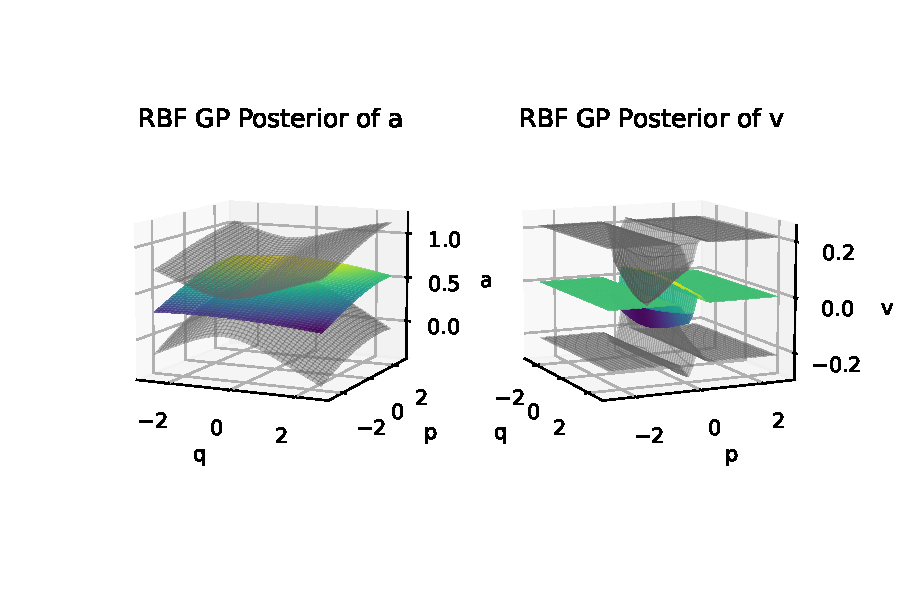
\includegraphics[width=\linewidth]{../codes/figures/posterior_pendulum_rbf.pdf}
        \caption{pendulum RBF posterior}
        \label{fig:posterior_pendulum_rbf}
     \end{subfigure}
     \hfill
     \begin{subfigure}[b]{\linewidth}
         \centering
         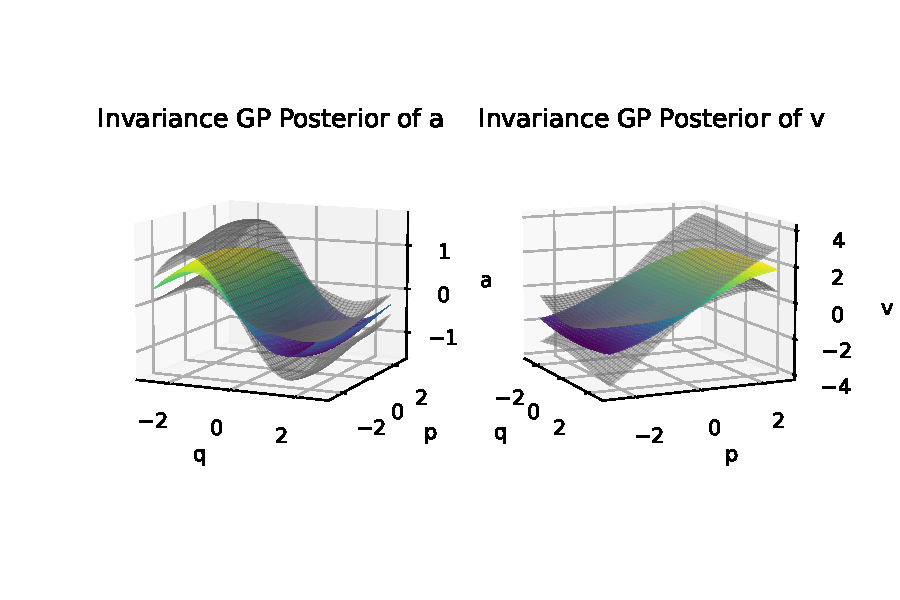
\includegraphics[width=\linewidth]{../codes/figures/posterior_pendulum_invariance.pdf}
         \caption{pendulum invariance posterior}
         \label{fig:posterior_pendulum_invariance}
     \end{subfigure}
        \caption{pendulum posteriors}
        \label{fig:posterior_pendulum}
\end{figure}



From table \ref{tab:pendulum_performance}, figure \ref{fig:pendulum_prediction}, \ref{fig:pendulum_energy}.
This time, again the RBF kernel performs poorly.
The known kernel performs very well again, almost exactly the same as the ground truth.
However, this time, the learnt invariance is slightly worse; this is expected since we are approximating a sine function with a cubic polynomial, and so some level of deviation is expected.
As we can see from figure \ref{fig:pendulum_learnt}, the learning is pretty accurate.
From the posteriors in \ref{fig:posterior_pendulum}, we see RBF generalise much better due to extra data points, but it is still very far from giving a reasonable prediction. 


\section{Invariance Density}
Here we will to explore how different invariance density affect the performance of the kernel as well as the degree of freedom.
Since 1D SHM is trival to learn, we test it on the nonlinear pendulum case, which will illustrate the point better. 
We will use different invariance density using the same training data and three different trajectories of testing data.
We again calculate the MSE of trajectory prediction as well as the percentage of energy deviation from the starting point of three different trajectories and average over.
The results is shown in figure \ref{fig:vary_invariance_density}.

\begin{figure}[H] 
  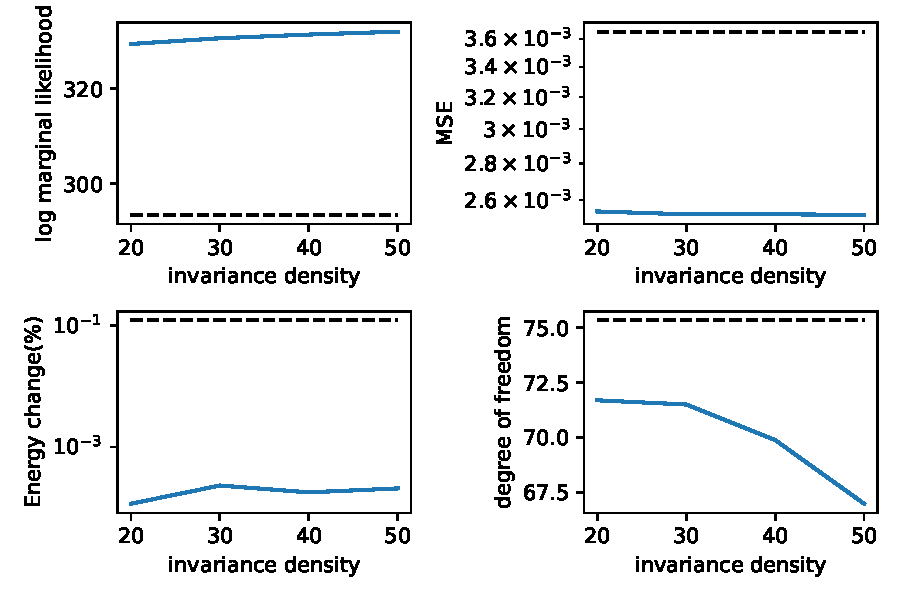
\includegraphics[width=0.8\linewidth]{../codes/figures/vary_invariance.pdf}
  \centering
  \caption{Effect of varying invariance density}
  \label{fig:vary_invariance_density}
\end{figure}

We can see that for the marginal likelihood, it increases as the number of invariance points increases, which is expected since we have more information/evidence to support the data.
However, MSE first decreases then increases.
The first decrease makes sense since with more invariance points, we should in principle predict better.
However, the increase is counter-intuitive.
We conclude that there is actually not that big a difference and it is possibly due to the numerical instability as we increase the size of the matrix with increasing invariance density.  
We also see the deviation of energy decreases as we increase the number of invariance points, which makes sense because we are imposing "more" invariance in the input space by increasing the invariance density.
Lastly, we see the degree of freedom does not vary much either, while in theory it should decrease with increasing invariance density due to more constraints on the function.

Overall, we see there is not that big an advantage to increase our invariance density beyond a certain point due to diminishing return in performance and $N^6$ computational cost.
Therefore, from this point we will choose the smallest invariance density that give reasonable performance.  

\section{Effect of Jitter}
Since we need a little bit of jitter to stabilise the computation of our invariance kernel as explained above, and that adding jitter is the same as adding noise to the invariance (since we are adding it on the diagonal of $LKL^T$ submatrix), we need to make sure it is not too large and too noisy, which will destroy the point of having invariance to start with. 
So we will again assess the performance in the similar way as above using different amount of jitter.
The results is shown in figure \ref{fig:vary_jitter}.

\begin{figure}[H] 
  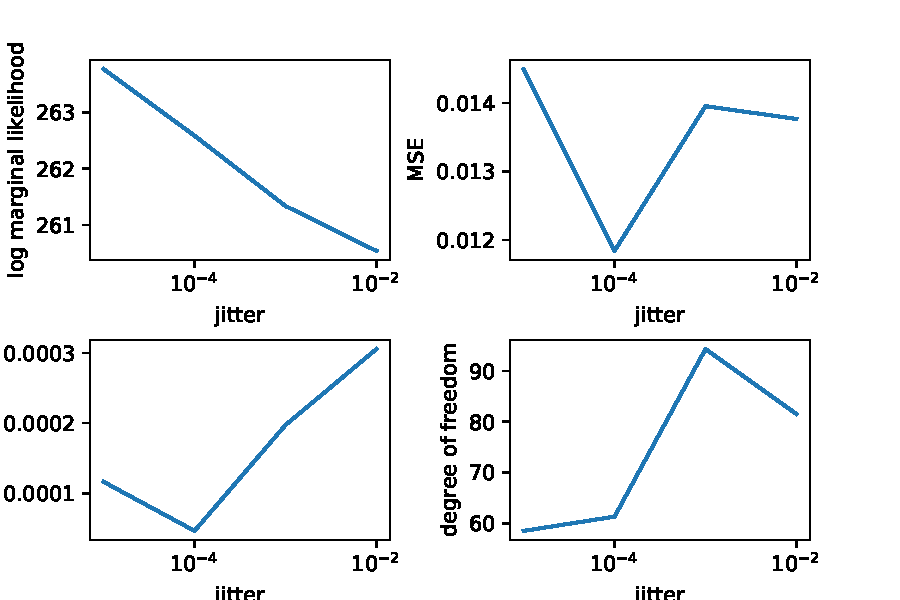
\includegraphics[width=0.8\linewidth]{../codes/figures/vary_jitter.pdf}
  \centering
  \caption{Effect of varying jitter}
  \label{fig:vary_jitter}
\end{figure}

For marginal likelihood, we see it decreases as jitter increases as expected because then the invariance is not as strong a contraint.
For MSE, we expect to see steady decrease in performance.
However, here we see a dip initially.
Again, there is not a big difference, and that the lowest jitter might not be enough to stablise the model so that the worse performance could be due to numerical instability.
We see a similar pattern in energy conservation, where we see energy consevation is not as enforced when we have noisy invariance.
Degree of freedom increases with jitter as expected since we are relaxing the constraints.
While the lower the jitter, the higher the performance should be in theory; the instability of matrix inversion and numerical errors could cause a drop in performance.
As a result,  we will also choose the smallest amount of jitter that still gives stable performance.  
Note that, in both cases of varying jitter and invariance density; all of them are much better than the RBF in performance anyways.

\section{Damped SHM}
For damped system, we have exactly the same setup as the original undamped SHM.
The results is again summarised in table \ref{tab:damped_shm_performance} and figure \ref{fig:damped_shm_prediction}, \ref{fig:damped_shm_energy}.
The learnt $f(p)$ and $g(q)$ is shown in figure \ref{fig:damped_shm_learnt}.

\begin{table}[H]
  \centering
  \begin{tabular}{l l l l}
    \hline
Method           & RBF & Known Invariance&  Learnt Invariance\\
  \hline
    Log Marginal Likelihood & 67.69 & 74.84 & 77.43  \\
MSE & 0.9226 & 0.4772 & 0.2405 \\
    \hline
  \end{tabular}
  \caption{Damped SHM performance}
  \label{tab:damped_shm_performance}
\end{table}

\begin{figure}[H]
        \centering
        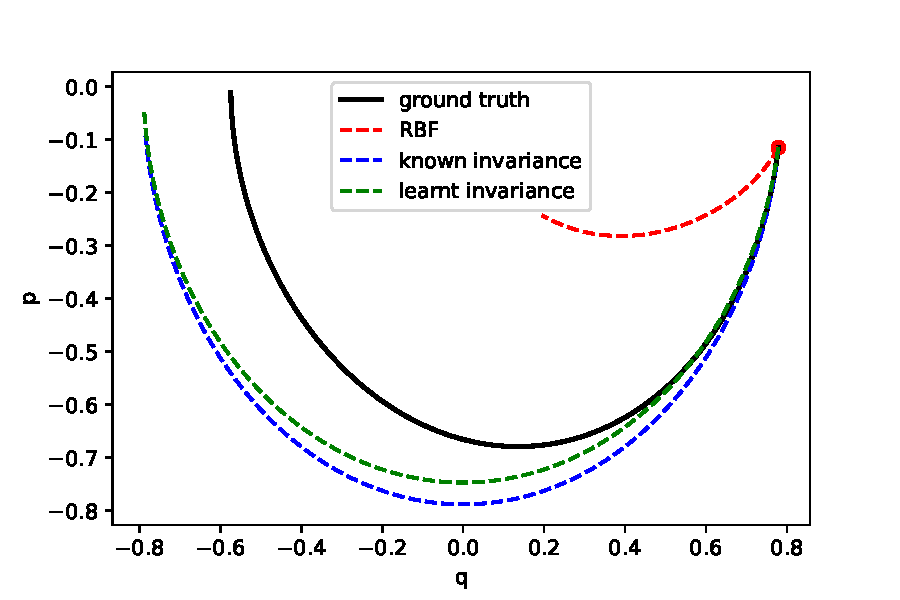
\includegraphics[width=0.8\linewidth]{../codes/figures/damped_shm_predicted.pdf}
        \caption{Damped SHM predicted trajectory}
        \label{fig:damped_shm_prediction}
\end{figure}

\begin{figure}[H] 
  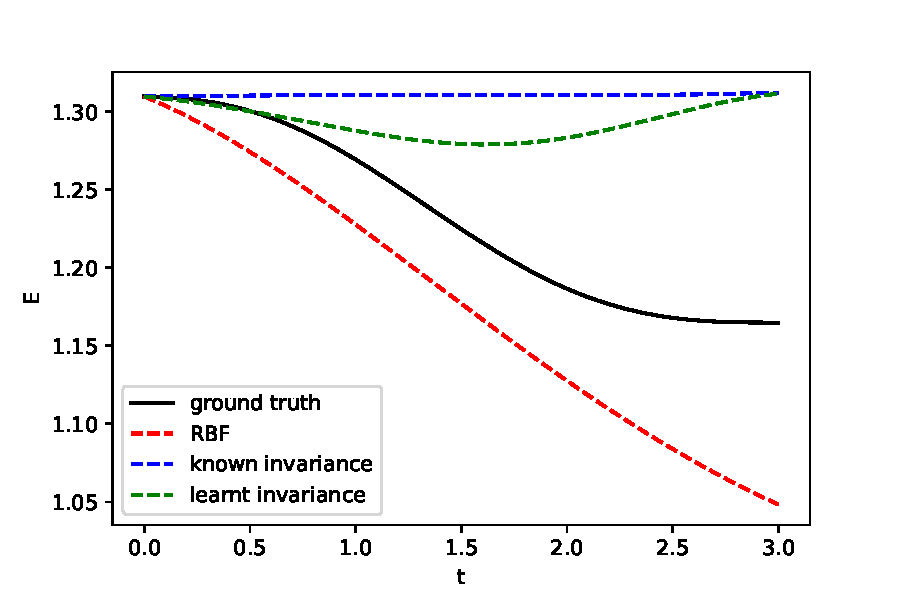
\includegraphics[width=0.8\linewidth]{../codes/figures/damped_shm_energy.pdf}
  \centering
  \caption{Energy conservation for damped SHM}
  \label{fig:damped_shm_energy}
\end{figure}


\begin{figure}[H] 
  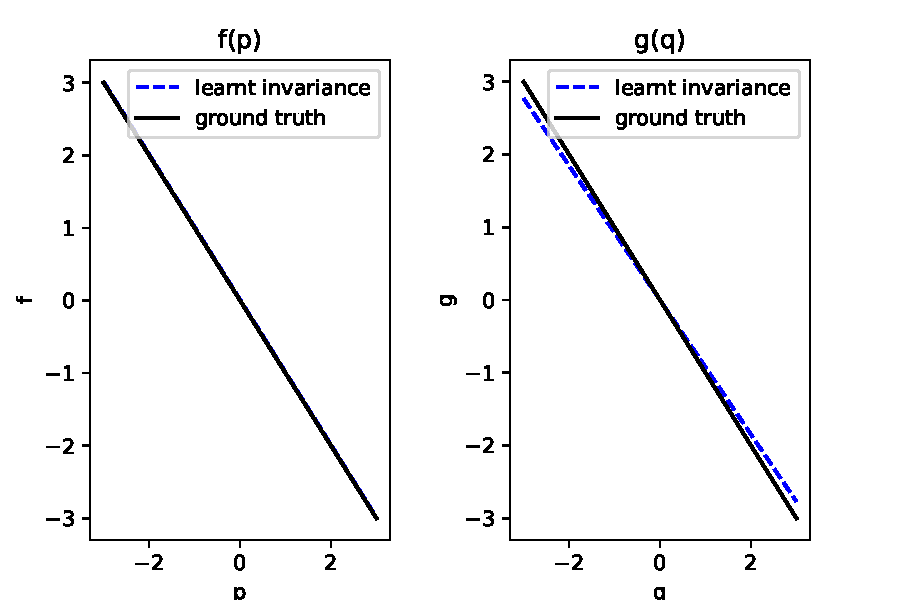
\includegraphics[width=0.8\linewidth]{../codes/figures/damped_shm_learnt.pdf}
  \centering
  \caption{Learnt invariance for damped SHM}
  \label{fig:damped_shm_learnt}
\end{figure}

We can see that the RBF performance is still poor as before.
However, this time the invariance kernel does not perform as well as before. 
This is expected since we still enforce some degree of invariance, even though it is noisy. 
However, it is clear that it is making use of the knowledge of the invariance since the performance is fairly good.
For energy consevation, it is reassuring that the invariance kernel is still remains invariant, while the learnt invariance might deviate a little since the extra parameters in the polynomial might fit to the damped data; but overall it conserves energy relatively well compare to the ground truth.
Also, when we are learning the invariance, it again successfully recover the physics even under the effect of damping.

\section{Damped Pendulum}
Again, the setting of damped pendulum is the same as the undamped pendulum.
The results is summarised in table \ref{tab:damped_pendulum_performance} and figure \ref{fig:damped_pendulum_prediction}, \ref{fig:damped_pendulum_energy}.
With the learnt polynomial in \ref{fig:damped_pendulum_learnt}.

\begin{table}[H]
  \centering
  \begin{tabular}{l l l l}
    \hline
Method           & RBF & Known Invariance&  Learnt Invariance\\
  \hline
Log Marginal Likelihood & 229.96 & 243.41 & 243.48  \\
MSE & 0.5983 & 0.0323 & 0.0877 \\
    \hline
  \end{tabular}
  \caption{Damped Pendulum Performance}
  \label{tab:damped_pendulum_performance}
\end{table}

\begin{figure}[H]
        \centering
        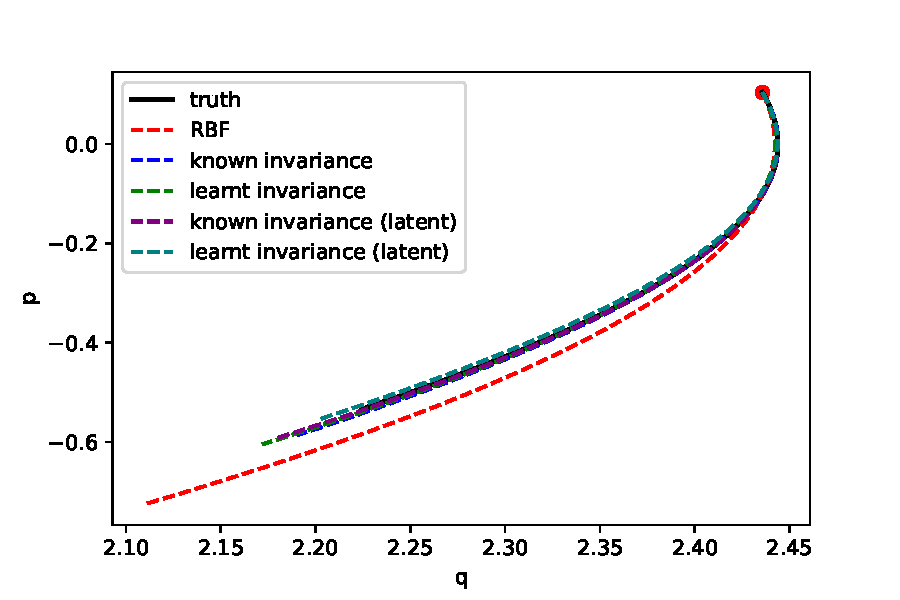
\includegraphics[width=0.8\linewidth]{../codes/figures/damped_pendulum_predicted.pdf}
        \caption{damped pendulum predicted trajectory}
        \label{fig:damped_pendulum_prediction}
\end{figure}

\begin{figure}[H] 
  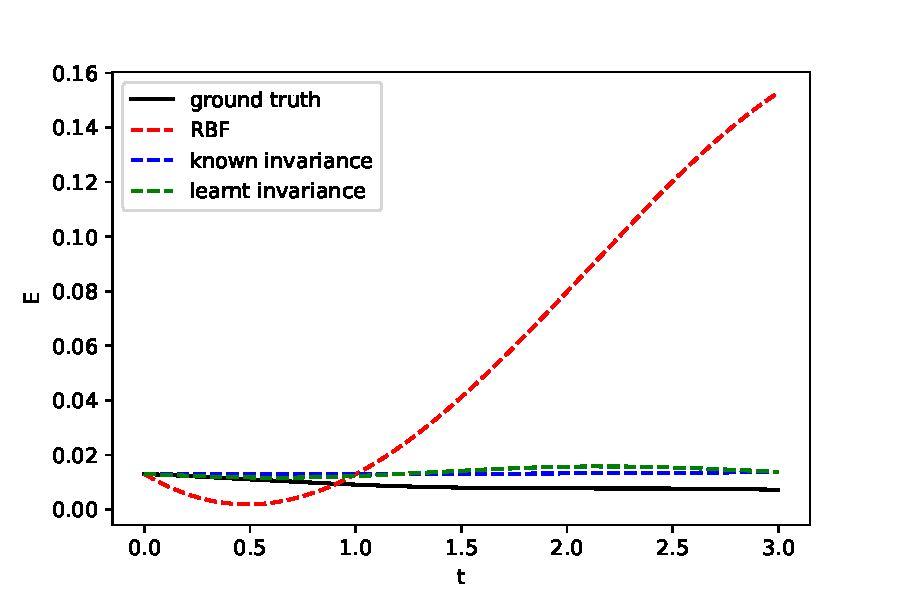
\includegraphics[width=0.8\linewidth]{../codes/figures/damped_pendulum_energy.pdf}
  \centering
  \caption{Energy conservation for damped pendulum}
  \label{fig:damped_pendulum_energy}
\end{figure}


\begin{figure}[H] 
  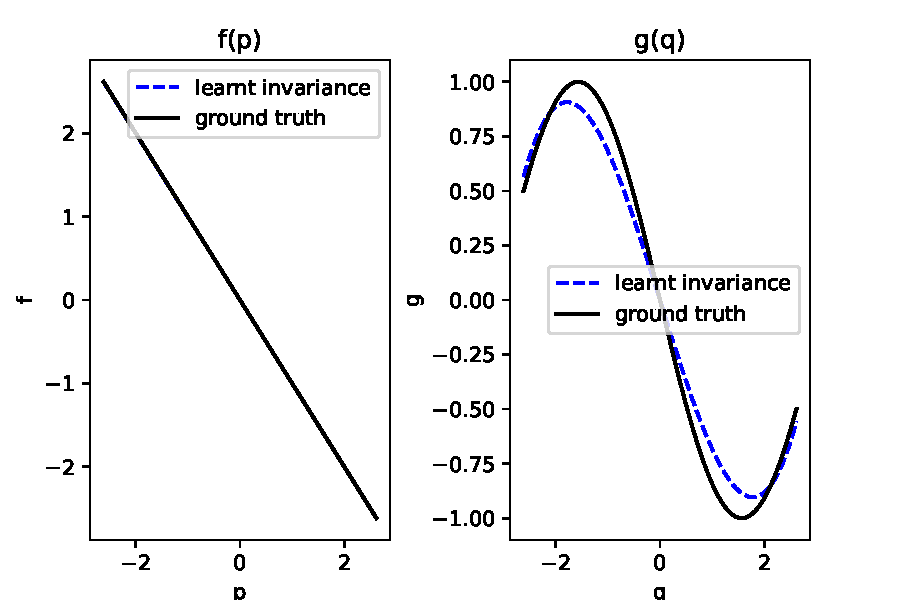
\includegraphics[width=0.8\linewidth]{../codes/figures/damped_pendulum_learnt.pdf}
  \centering
  \caption{Learnt invariance for damped pendulum}
  \label{fig:damped_pendulum_learnt}
\end{figure}

We see similar performance as in damped SHM, with invariance kernels performs slightly worse than undamped version but still much better than the RBF.
The energy conservation still holds mostly for invariance kernels.
However, this time, the learnt polynomial is not as good as the undamped case with much more deviation; this is expected due to the damping.

\section{2D SHM}
Here we again use the same set of input space as the 1D space, but double the dimensions. 
Here we actaully have the input space of $q_1, q_2$ being between $\pm 5$ and $p_1, p_2$ between $\pm 0.5$. 
This is done so that when we scale the data with MinMax scaler, the points will be less clustered.
We use 30 points in this setting.
\textbf{One very important note} is that when we are learning invariance, we initialise the hyperparameters of the base RBF kernel (lengthscales and variance local grids as well as likelihood variance) at the values trained by the known invariance.
We also intialise the polynomial coefficients at the true theoretical values.
These are done due to the fact the optimiser is often stuck at local minima.
We intialise the values there so that if it is indeed the true invariance, the optimiser should regonise it and not optimise too much since that is roughly the true minimum.
Therefore, we would expect to get similar performance and marginal likelihood.

The results are summarised in table \ref{tab:SHM_2d_performance} and figure \ref{fig:shm_2d_prediction}, \ref{fig:shm_2d_energy}.
Since it is difficult to visualise 4 dimensional space, we will plot them individually.

\begin{table}[H]
  \centering
  \begin{tabular}{l l l l}
    \hline
Method           & RBF & Known Invariance&  Learnt Invariance\\
  \hline
Log Marginal Likelihood & 387.08 & 441.60 & 438.42  \\
MSE & 1.1252 & 0.7374 & 0.7359 \\
                    \hline
  \end{tabular}
  \caption{2D SHM Invariance performance}
  \label{tab:SHM_2d_performance}
\end{table}

\begin{figure}[H] 
  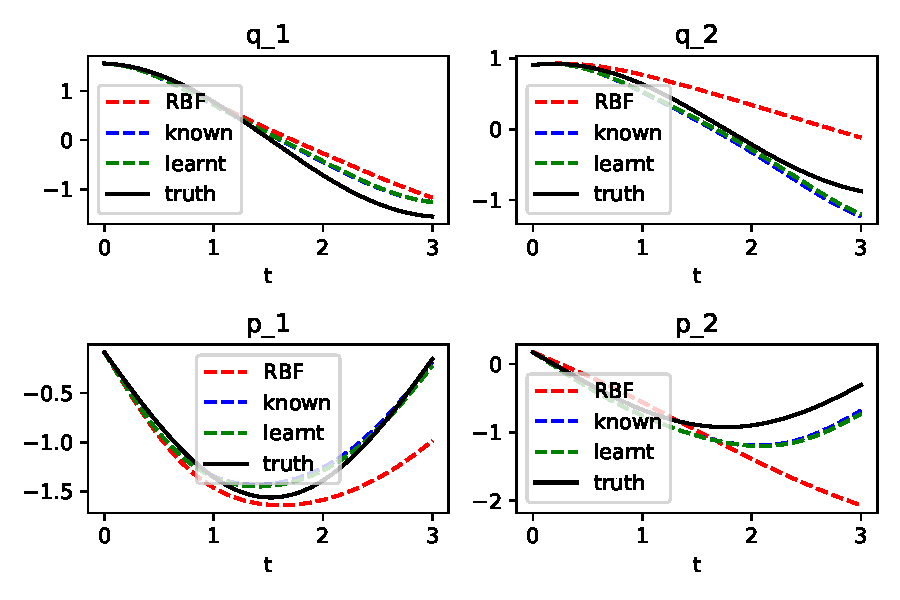
\includegraphics[width=0.8\linewidth]{../codes/figures/shm_2d_predicted.pdf}
  \centering
  \caption{2D SHM prediction}
  \label{fig:shm_2d_prediction}
\end{figure}

\begin{figure}[H] 
  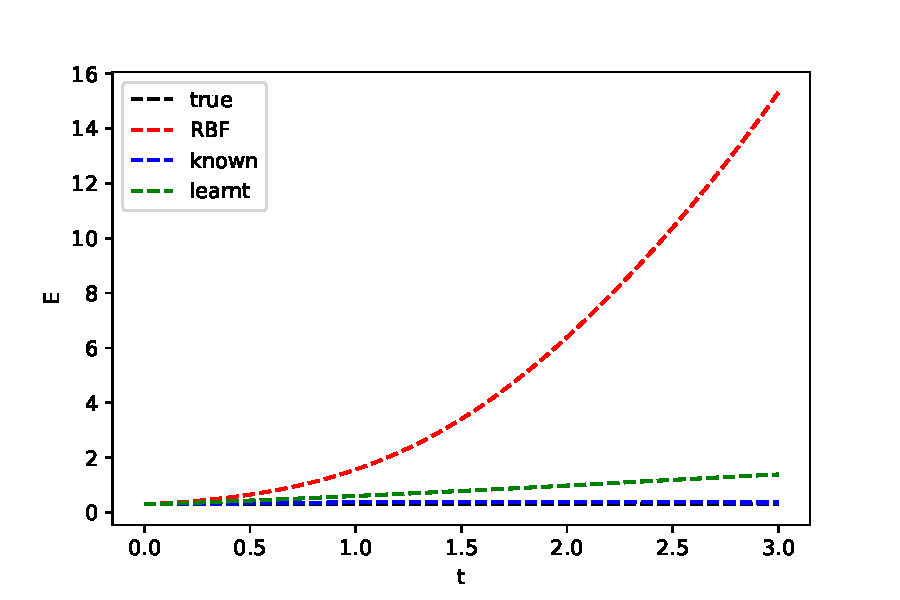
\includegraphics[width=0.8\linewidth]{../codes/figures/shm_2d_energy.pdf}
  \centering
  \caption{2D SHM energy}
  \label{fig:shm_2d_energy}
\end{figure}

Firstly, we can see that the invariance kernel still performs very well compared to RBF, although not as good as the 1D case as expected since higher dimensional problem is deemed to be more difficult.
We can see the learnt invariance again is almost exactly the same as the known form, which is reassuring.
Also, the conservation of energy is again pretty well obeyed.

\section{Double Pendulum}
With double pendulum, we have angles being between $\pm 60^\circ$ and angular velocity between $\pm 10^\circ$.
The results are summarised in table \ref{tab:double_pendulum_performance} and figure \ref{fig:double_pendulum_prediction}, \ref{fig:double_pendulum_energy}.
Again we used 30 points to train, but this time we do not use scaling since perhaps due to its nonlinear nature, it made the performance much worse by possibly modifying its underlying distribution.

\begin{table}[H]
  \centering
  \begin{tabular}{l l l l}
    \hline
Method           & RBF & Known Invariance&  Learnt Invariance\\
  \hline
Log Marginal Likelihood & 455.89 & 471.01 & 494.37  \\
MSE & 0.3879 & 0.0286 & 0.0362 \\
    \hline
  \end{tabular}
  \caption{Double pendulum invariance performance}
  \label{tab:double_pendulum_performance}
\end{table}

\begin{figure}[H] 
  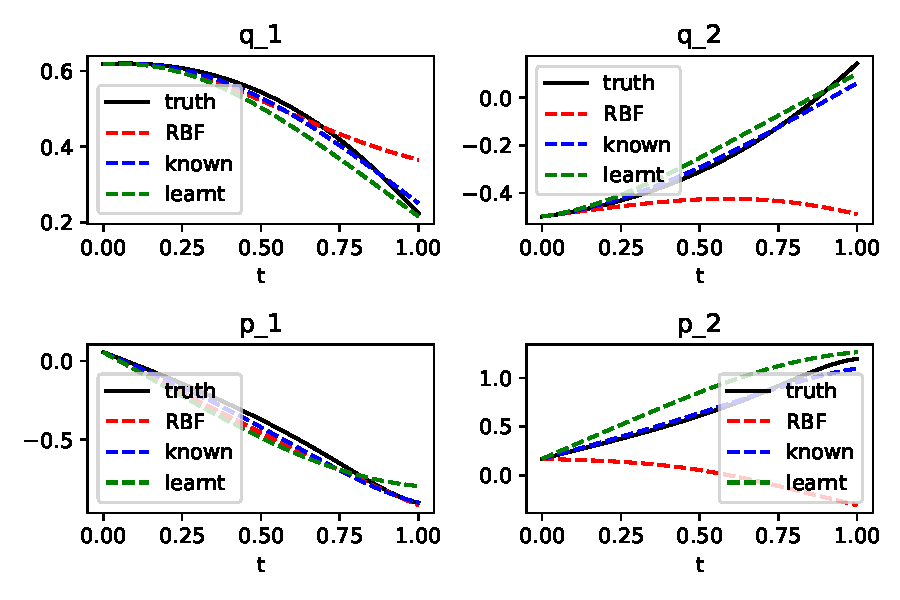
\includegraphics[width=0.8\linewidth]{../codes/figures/double_pendulum_predicted.pdf}
  \centering
  \caption{Double pendulum prediction}
  \label{fig:double_pendulum_prediction}
\end{figure}

\begin{figure}[H] 
  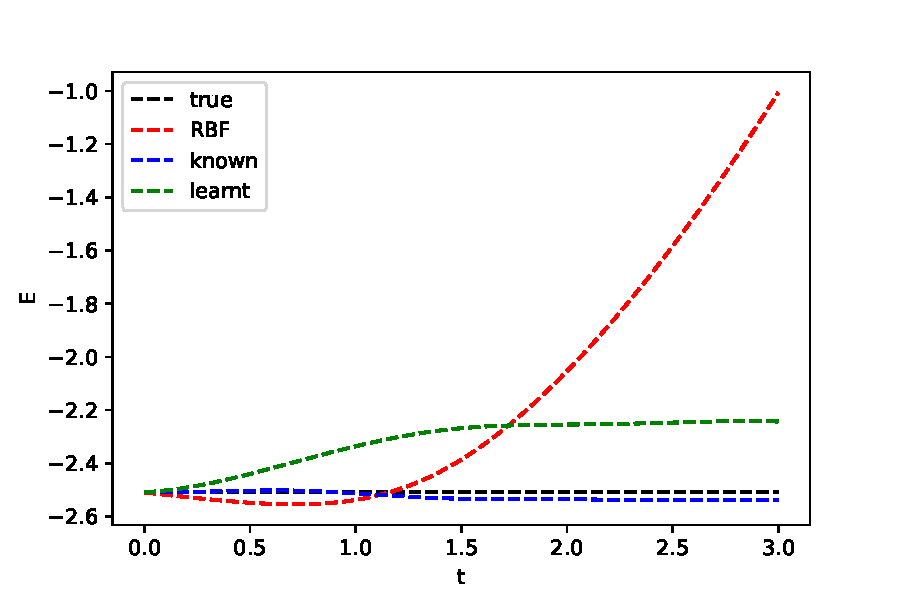
\includegraphics[width=0.8\linewidth]{../codes/figures/double_pendulum_energy.pdf}
  \centering
  \caption{Double pendulum energy}
  \label{fig:double_pendulum_energy}
\end{figure}
Now it is interesting to obsesrve that the marginal likelihood of the learnt form is even better than known form.
This is likely due to "overfitting" of the large number of parameters from the polynomials (140 in total).
Also, we are only expanding up to the cubic term, therefore we do not expect very good learning for the invariance.
However, in our case, the approximation is fairly good, possibly due to relatively small value of $q, p$ so the polynomial approximation is good.
Nevertheless, it is clear that there is still some errors with learning invariance from figure \ref{fig:double_pendulum_energy} since it only flattens toward the end of the trajectory.

\chapter{Conclusion}


Conclusion goes here. 


% References: modify the file refs.bib
\bibliographystyle{plainnat}
\bibliography{refs}


%\clearpage
% %% reset page counter and start appendix pages with A
%\pagenumbering{arabic}
%\renewcommand*{\thepage}{A\arabic{page}}
%\appendix
%
%\chapter{Appendix title}
%
%Appendix goes here.

\end{document}
